\documentclass[a4paper,12pt]{article}
\usepackage{indentfirst}
\usepackage[T1]{fontenc}
\usepackage{graphicx}
\usepackage{float}
\usepackage{caption}
\usepackage{amsmath}
\graphicspath{{../Imagens/}{Imagens/}}
\renewcommand{\figurename}{Figura}
\captionsetup{
  justification=raggedright,
  singlelinecheck=false,
  labelsep=endash,
  font=small,
  labelfont=bf,
  skip=6pt,
  position=above
}
\newcommand{\fonteelemento}[1]{%
  \par\smallskip
  {\footnotesize\raggedright Fonte: #1.\par}%
}

\begin{document}

\section{Desenvolvimento e Implementa\c{c}\~ao}


Este cap\'itulo apresenta a implementa\c{c}\~ao da plataforma, desde a organiza\c{c}\~ao dos recursos f\'isicos at\'e a integra\c{c}\~ao dos m\'odulos funcionais. A descri\c{c}\~ao foi conferida diretamente na vers\~ao corrente do firmware em \texttt{Codigos/IDroid/main}; documentos hist\'oricos foram usados apenas para contextualizar decis\~oes de desenvolvimento e n\~ao como autoridade sobre a vers\~ao integrada.


\subsection{Vis\~ao geral do sistema}


A plataforma foi organizada em quatro n\'iveis: hardware, drivers, servi\c{c}os compartilhados e m\'odulos funcionais. O hardware re\'une o XIAO ESP32-C6, o Round Display e os sensores. Os drivers encapsulam os protocolos e registradores de cada dispositivo. Os servi\c{c}os coordenam recursos utilizados por mais de um m\'odulo, como I$^2$C, LVGL e NVS. Os m\'odulos associam aquisi\c{c}\~ao, processamento, estado funcional e tela.


A Figura~\ref{fig:arquitetura-implementada} sintetiza os componentes confirmados e as dire\c{c}\~oes de controle, dados e acesso ao hardware.


\begin{figure}[H]
\centering
\caption{Arquitetura de componentes da plataforma implementada}
\label{fig:arquitetura-implementada}
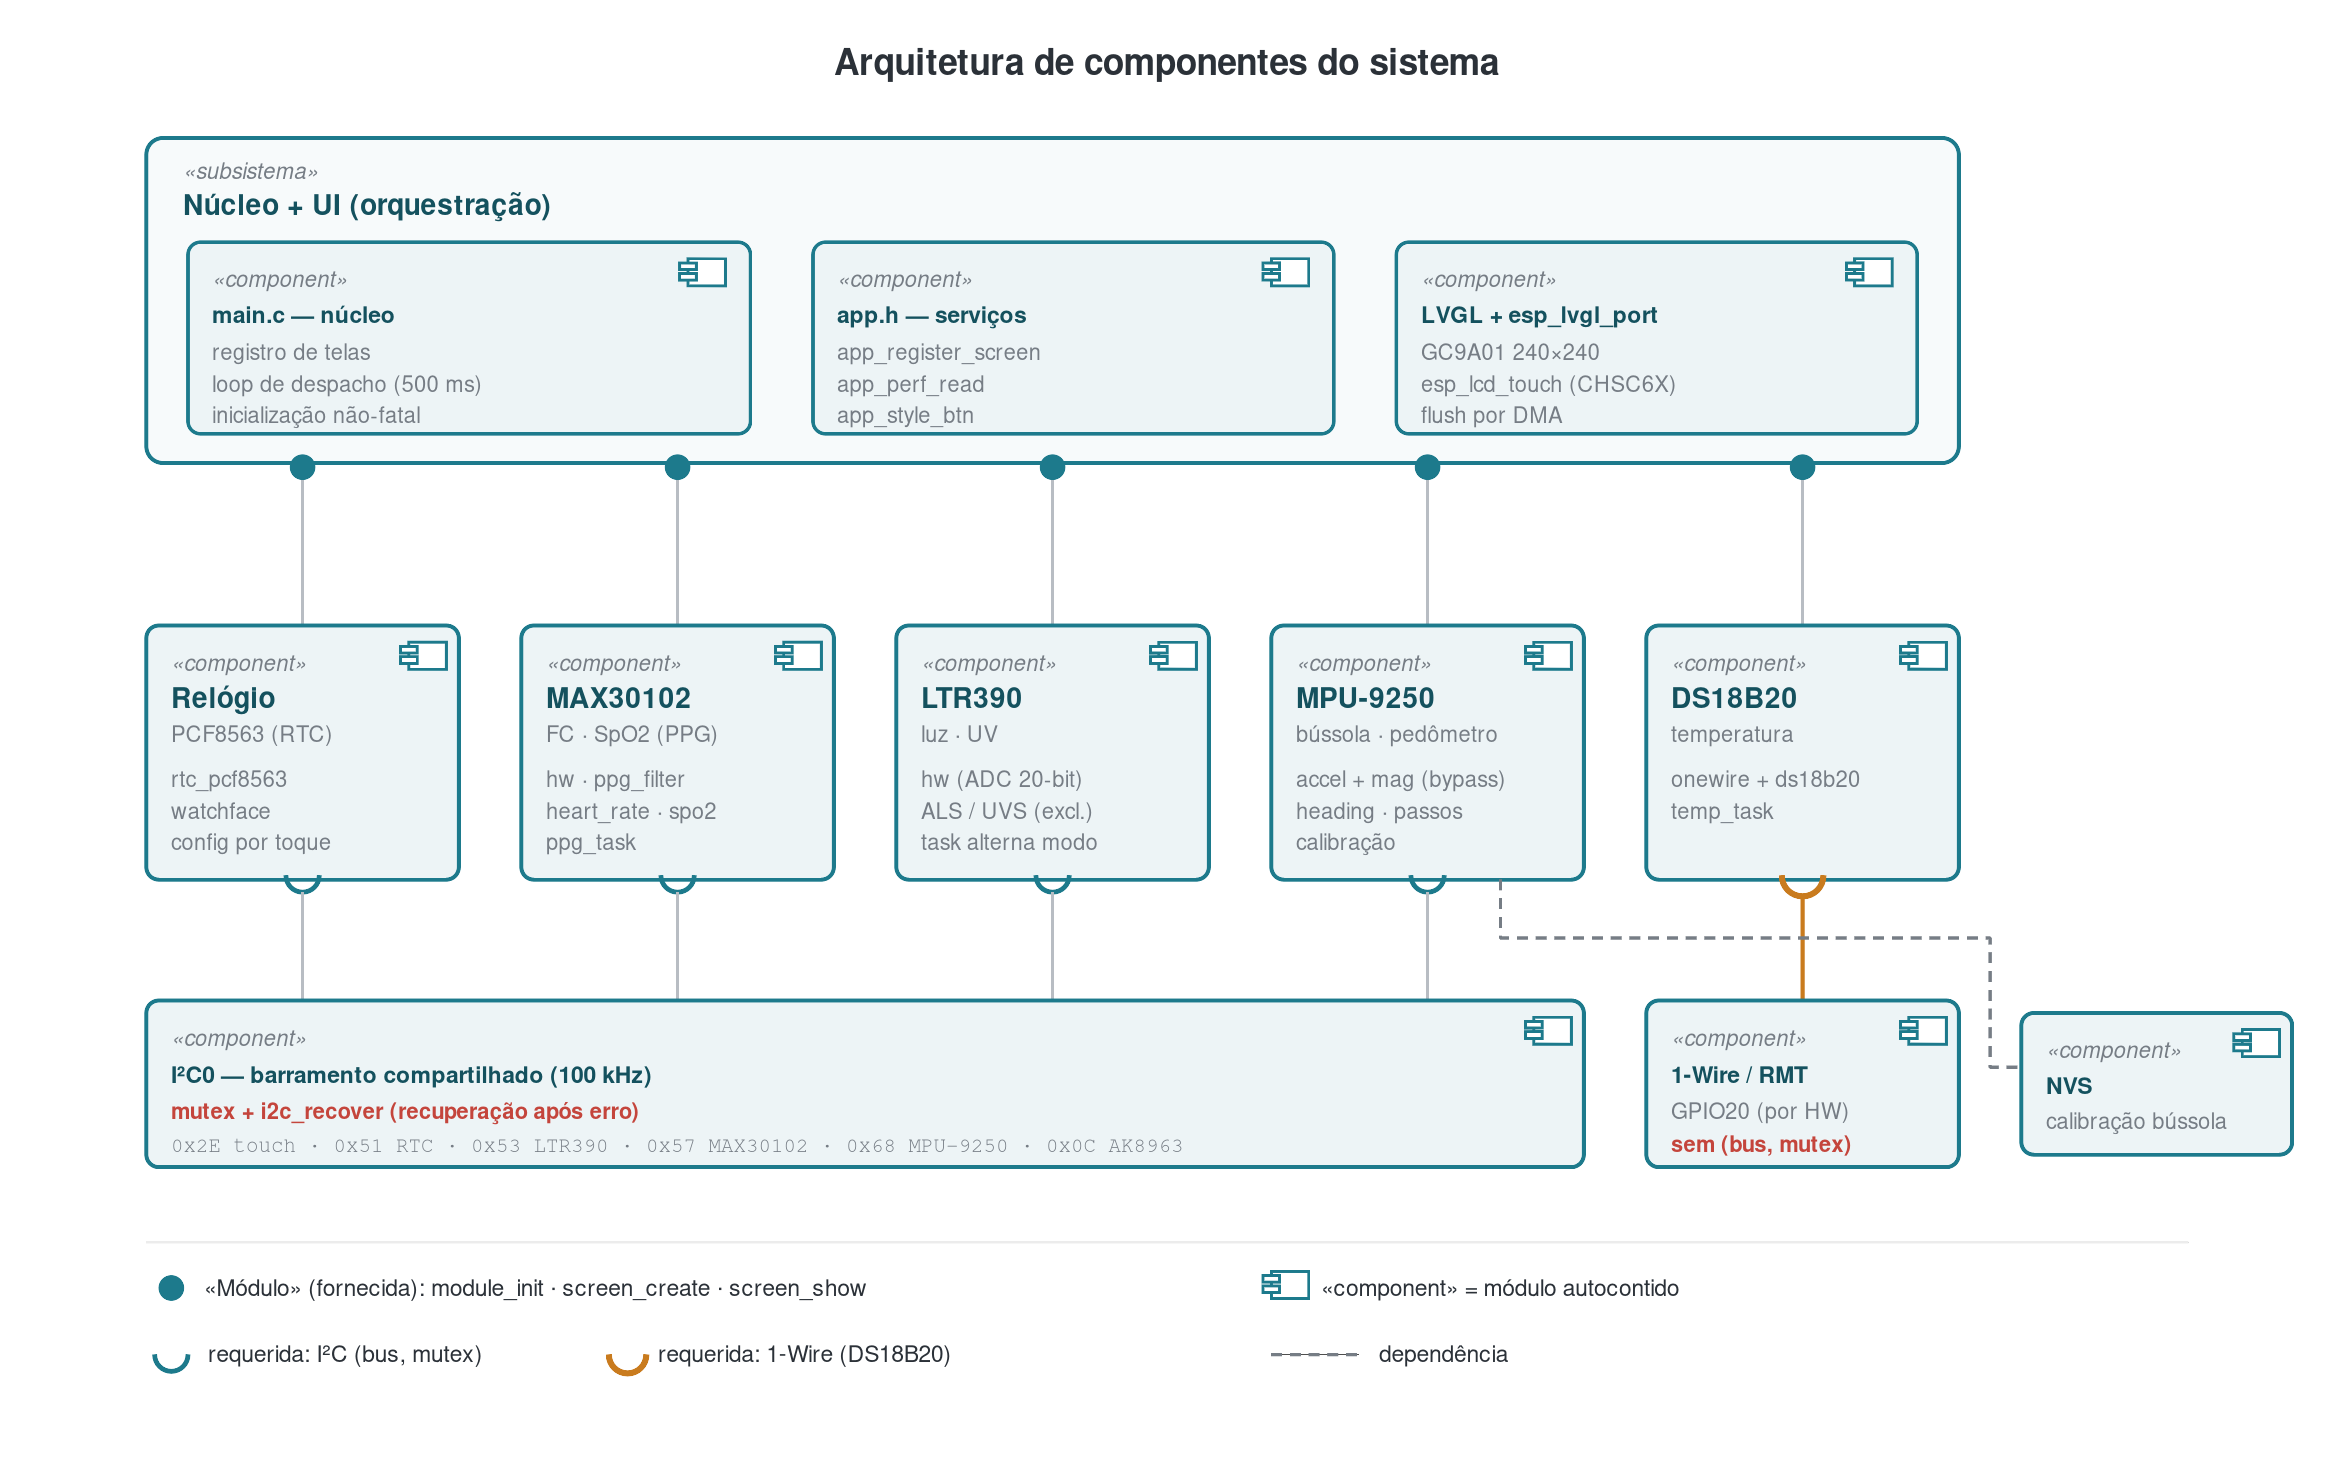
\includegraphics[width=0.96\textwidth]{Diagramas/sistema/arquitetura_componentes_sistema.png}
\fonteelemento{Elaborado pelo autor a partir do firmware integrado}
\end{figure}


O n\'ucleo n\~ao executa os algoritmos de cada sensor. Ele inicializa os servi\c{c}os, solicita a inicializa\c{c}\~ao dos m\'odulos, cria as telas e despacha a atualiza\c{c}\~ao correspondente \`a tela ativa. A aquisi\c{c}\~ao peri\'odica permanece nas tarefas dos m\'odulos, enquanto a LVGL \'e manipulada segundo o mecanismo de exclus\~ao fornecido por sua porta para o ESP-IDF.


\subsection{Arquitetura de hardware}


\subsubsection{Barramento I$^2$C compartilhado}


O I$^2$C foi criado uma \'unica vez pelo n\'ucleo com a API mestre introduzida nas vers\~oes recentes do ESP-IDF. O barramento opera a 100 kHz em SDA GPIO22 e SCL GPIO23. Cada driver registra seu dispositivo l\'ogico nessa inst\^ancia, em vez de criar um controlador pr\'oprio.


Seis endere\c{c}os coexistem no barramento: CHSC6X em 0x2E, PCF8563 em 0x51, LTR390 em 0x53, MAX30102 em 0x57, MPU-9250 em 0x68 e AK8963 em 0x0C. O \'ultimo torna-se acess\'ivel externamente quando o MPU-9250 \'e colocado em modo \emph{bypass}. Embora perten\c{c}am ao mesmo encapsulamento funcional, MPU-9250 e AK8963 constituem alvos I$^2$C distintos.


A frequ\^encia de 100 kHz foi adotada na integra\c{c}\~ao, substituindo configura\c{c}\~oes mais altas usadas em testes isolados. A redu\c{c}\~ao aumenta a margem para os tempos de subida na montagem com fios e m\'ultiplas placas. Como todos os dispositivos compartilham o controlador e as linhas, a coordena\c{c}\~ao por software e a recupera\c{c}\~ao do barramento foram tratadas como servi\c{c}os sist\^emicos.


\subsubsection{Interface SPI}


O display GC9A01A utiliza o perif\'erico SPI2 a 40 MHz. As linhas de clock e dados s\~ao compartilh\'aveis com o slot microSD do Round Display, enquanto sinais de sele\c{c}\~ao independentes delimitam as transa\c{c}\~oes. O firmware integrado utiliza o controlador de LCD disponibilizado como componente do ecossistema ESP-IDF; o cart\~ao n\~ao integra as fun\c{c}\~oes avaliadas.


As transfer\^encias gr\'aficas s\~ao predominantemente unidirecionais, do ESP32-C6 para o controlador. O uso de DMA pela porta gr\'afica permite transferir blocos de pixels sem movimenta\c{c}\~ao individual pela CPU. O acesso ao display permanece encapsulado pelo driver e pela LVGL, de modo que m\'odulos funcionais criam objetos gr\'aficos sem iniciar transa\c{c}\~oes SPI diretamente.


\subsubsection{Interface 1-Wire/RMT}


O DS18B20 utiliza uma interface separada, no GPIO20, com resistor de \emph{pull-up} externo. Os intervalos do protocolo 1-Wire s\~ao produzidos e amostrados por meio do perif\'erico RMT. Essa solu\c{c}\~ao reduz a depend\^encia de atrasos ativos em software e evita que a temporiza\c{c}\~ao de cada bit dependa diretamente da execu\c{c}\~ao cont\'inua de uma tarefa.


Foram reutilizados os componentes oficiais \texttt{onewire\_bus} e \texttt{ds18b20}. O m\'odulo de temperatura recebe valores j\'a convertidos pela API do componente e n\~ao conhece a representa\c{c}\~ao dos s\'imbolos do RMT. A separa\c{c}\~ao demonstra que o contrato funcional n\~ao exige que todos os m\'odulos utilizem o mesmo transporte.


\subsubsection{Alimenta\c{c}\~ao}


O prot\'otipo pode ser alimentado por USB por meio do XIAO ESP32-C6 ou por bateria conectada ao circuito do Round Display. A vers\~ao implementada n\~ao inclui gerenciamento avan\c{c}ado de energia, e o backlight permanece ligado durante a opera\c{c}\~ao. Recursos de suspens\~ao profunda, controle de brilho e otimiza\c{c}\~ao de autonomia n\~ao fazem parte do desenvolvimento descrito.

A leitura da tens\~ao da bateria tamb\'em integra a vers\~ao final. O positivo ap\'os a chave alimenta um divisor 1:2 formado por dois resistores de $100~\mathrm{k}\Omega$; o ponto m\'edio segue para o GPIO0/A0 do XIAO ESP32-C6. O firmware aplica calibra\c{c}\~ao do ADC, m\'edia de 16 amostras e suaviza\c{c}\~ao temporal antes de apresentar o estado estimado. A Figura~\ref{fig:divisor-bateria-xiao} mostra o circuito efetivamente empregado. Como a estimativa se baseia em tens\~ao, ela n\~ao equivale a um contador de carga.

\begin{figure}[H]
\centering
\caption{Divisor resistivo empregado na leitura da tens\~ao da bateria}
\label{fig:divisor-bateria-xiao}
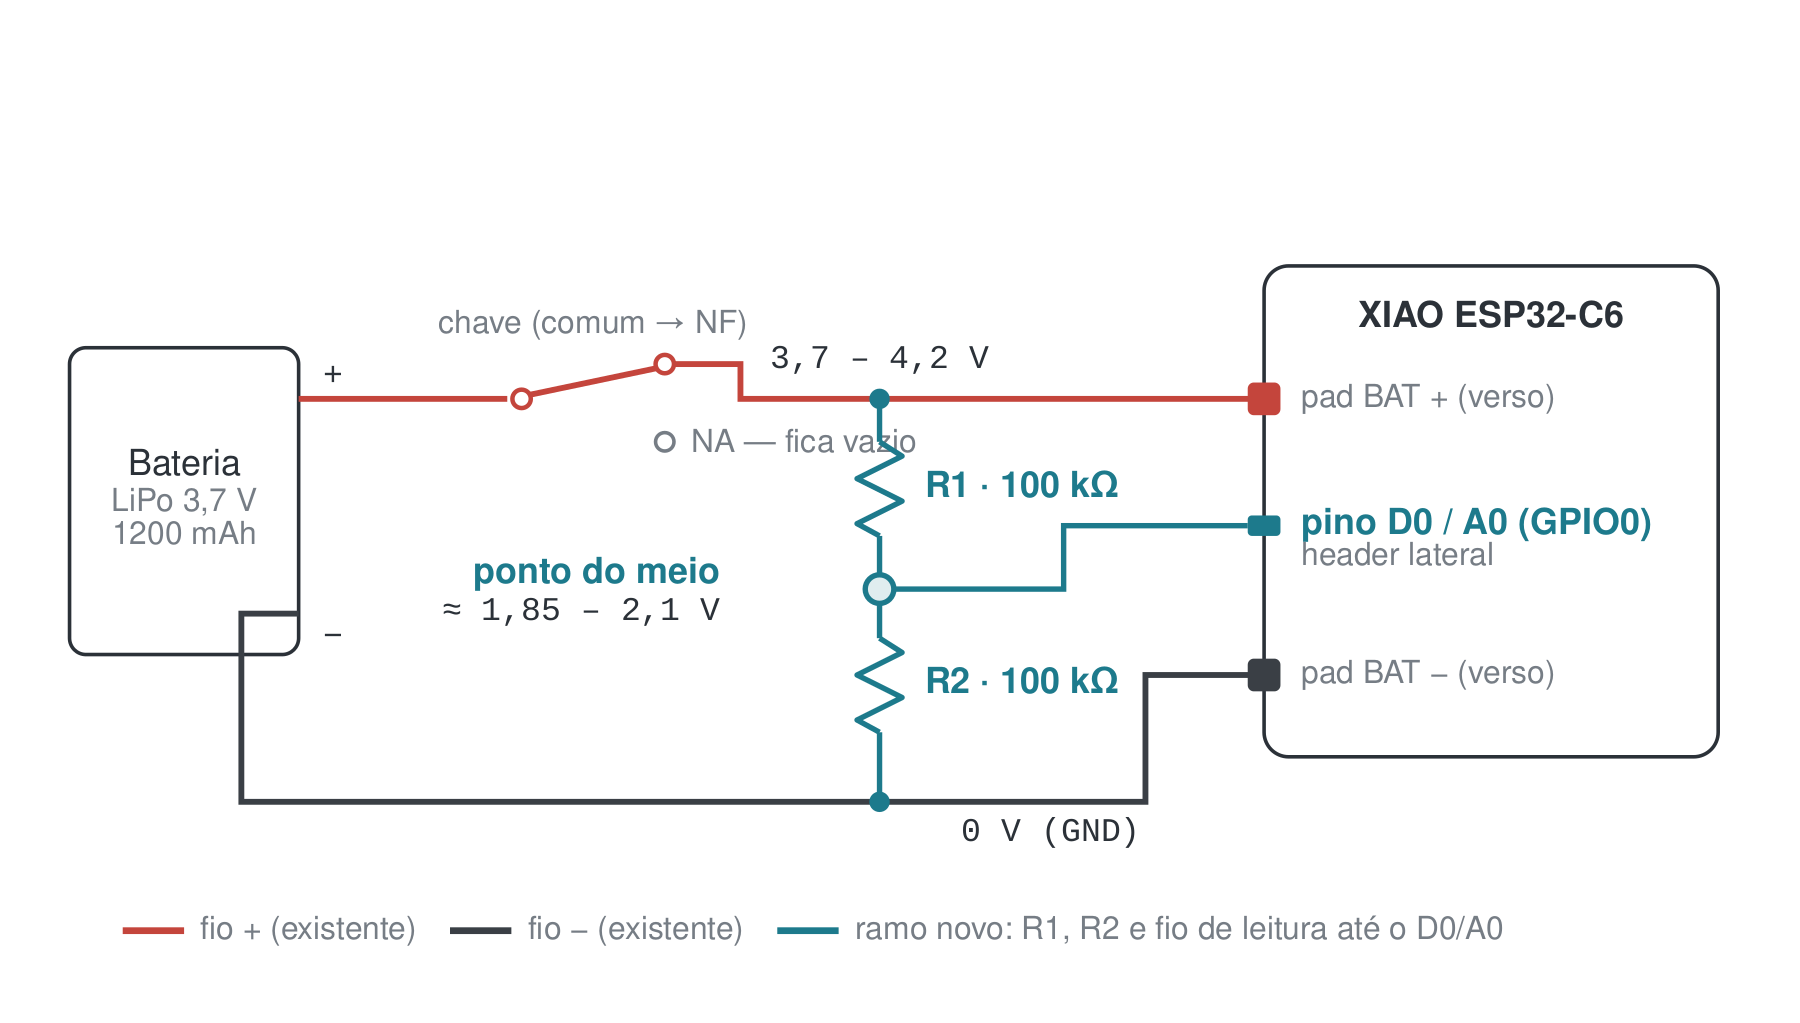
\includegraphics[width=0.90\textwidth]{Diagramas/bateria/divisor_bateria_xiao.png}
\fonteelemento{Elaborado pelo autor a partir do circuito implementado e de \texttt{bateria.c}}
\end{figure}


Durante a integra\c{c}\~ao, a alimenta\c{c}\~ao do MAX30102 exigiu aten\c{c}\~ao por causa dos pulsos de corrente dos emissores. Os testes A/B registrados no pr\'oprio c\'odigo associaram a configura\c{c}\~ao anterior, de aproximadamente 14,2 mA por emissor, a afundamento da linha de 3,3 V e travamento do I$^2$C na placa final. A configura\c{c}\~ao integrada passou a empregar o valor 0x24, correspondente a aproximadamente 7,2 mA por emissor.


\subsubsection{Placa prot\'otipo e inv\'olucro}


A integra\c{c}\~ao deixou a protoboard de desenvolvimento e foi transferida para uma placa prot\'otipo autoral, cujo esquema, leiaute, renderiza\c{c}\~oes e registro fotogr\'afico foram preservados. Um inv\'olucro tamb\'em foi fabricado por impress\~ao 3D para acomodar o conjunto. Esses elementos pertencem \`a implementa\c{c}\~ao realizada; revis\~oes futuras podem aprimor\'a-los, mas n\~ao correspondem a atividades pendentes de constru\c{c}\~ao.


\subsection{Arquitetura de software}


\subsubsection{Organiza\c{c}\~ao do firmware}


O firmware foi dividido por responsabilidade. O n\'ucleo cont\'em o ponto de entrada, os registros da aplica\c{c}\~ao e os servi\c{c}os comuns. Os drivers tratam comunica\c{c}\~ao e configura\c{c}\~ao dos circuitos integrados. Cada fun\c{c}\~ao apresentada ao usu\'ario re\'une os arquivos de seu m\'odulo, seu processamento e sua tela. Recursos gr\'aficos reutiliz\'aveis permanecem em uma camada de interface.


No diret\'orio \texttt{main}, o arquivo \texttt{main.c} concentra inicializa\c{c}\~ao, menus e despacho; \texttt{app.h} exp\~oe os servi\c{c}os comuns da aplica\c{c}\~ao; \texttt{i2c\_recover.c} encapsula a recupera\c{c}\~ao do barramento; \texttt{relogio/} cont\'em RTC, configura\c{c}\~ao, bateria e tela principal; \texttt{sensores/} separa os m\'odulos por dispositivo; e \texttt{ui/} preserva a base gr\'afica exportada. Dentro dos sensores, os sufixos \texttt{\_hw}, \texttt{\_process} e \texttt{\_screen} materializam, quando aplic\'avel, a separa\c{c}\~ao entre acesso ao dispositivo, tratamento e apresenta\c{c}\~ao.


O aspecto arquitetural relevante \'e a dire\c{c}\~ao das depend\^encias: os m\'odulos utilizam servi\c{c}os e drivers; o n\'ucleo utiliza suas interfaces p\'ublicas; e um m\'odulo funcional n\~ao acessa diretamente o estado interno de outro.


\subsubsection{Contrato uniforme de m\'odulo}


O contrato estabelece tr\^es etapas comuns: inicializar a fun\c{c}\~ao, criar sua tela e solicitar sua exibi\c{c}\~ao. Em forma abstrata, ele pode ser representado por:


\begin{verbatim}
[c]
esp_err_t modulo_init(/* depend\^encias necess\'arias */);
void modulo_screen_create(lv_obj_t *menu_origem);
void modulo_screen_show(void);
\end{verbatim}


A inicializa\c{c}\~ao prepara o driver, o estado e, quando necess\'ario, a tarefa de aquisi\c{c}\~ao. A cria\c{c}\~ao constr\'oi uma \'unica vez os objetos LVGL e registra a fun\c{c}\~ao que atualizar\'a a tela. A exibi\c{c}\~ao solicita a navega\c{c}\~ao para a tela j\'a criada.


A uniformidade refere-se ao ciclo de vida e \`as responsabilidades observ\'aveis, n\~ao \`a exig\^encia de assinaturas literalmente id\^enticas. M\'odulos I$^2$C recebem a refer\^encia do barramento e do mutex; o DS18B20 cria sua interface 1-Wire sem essas depend\^encias. Essa varia\c{c}\~ao conserva o transporte dentro do m\'odulo sem obrigar o n\'ucleo a simular uma depend\^encia inexistente.


A Figura~\ref{fig:ciclo-vida-modulo} mostra como o mesmo ciclo preserva uma tela informativa tanto no caminho dispon\'ivel quanto no caminho de sensor ausente.


\begin{figure}[H]
\centering
\caption{Ciclo de vida dos m\'odulos funcionais}
\label{fig:ciclo-vida-modulo}
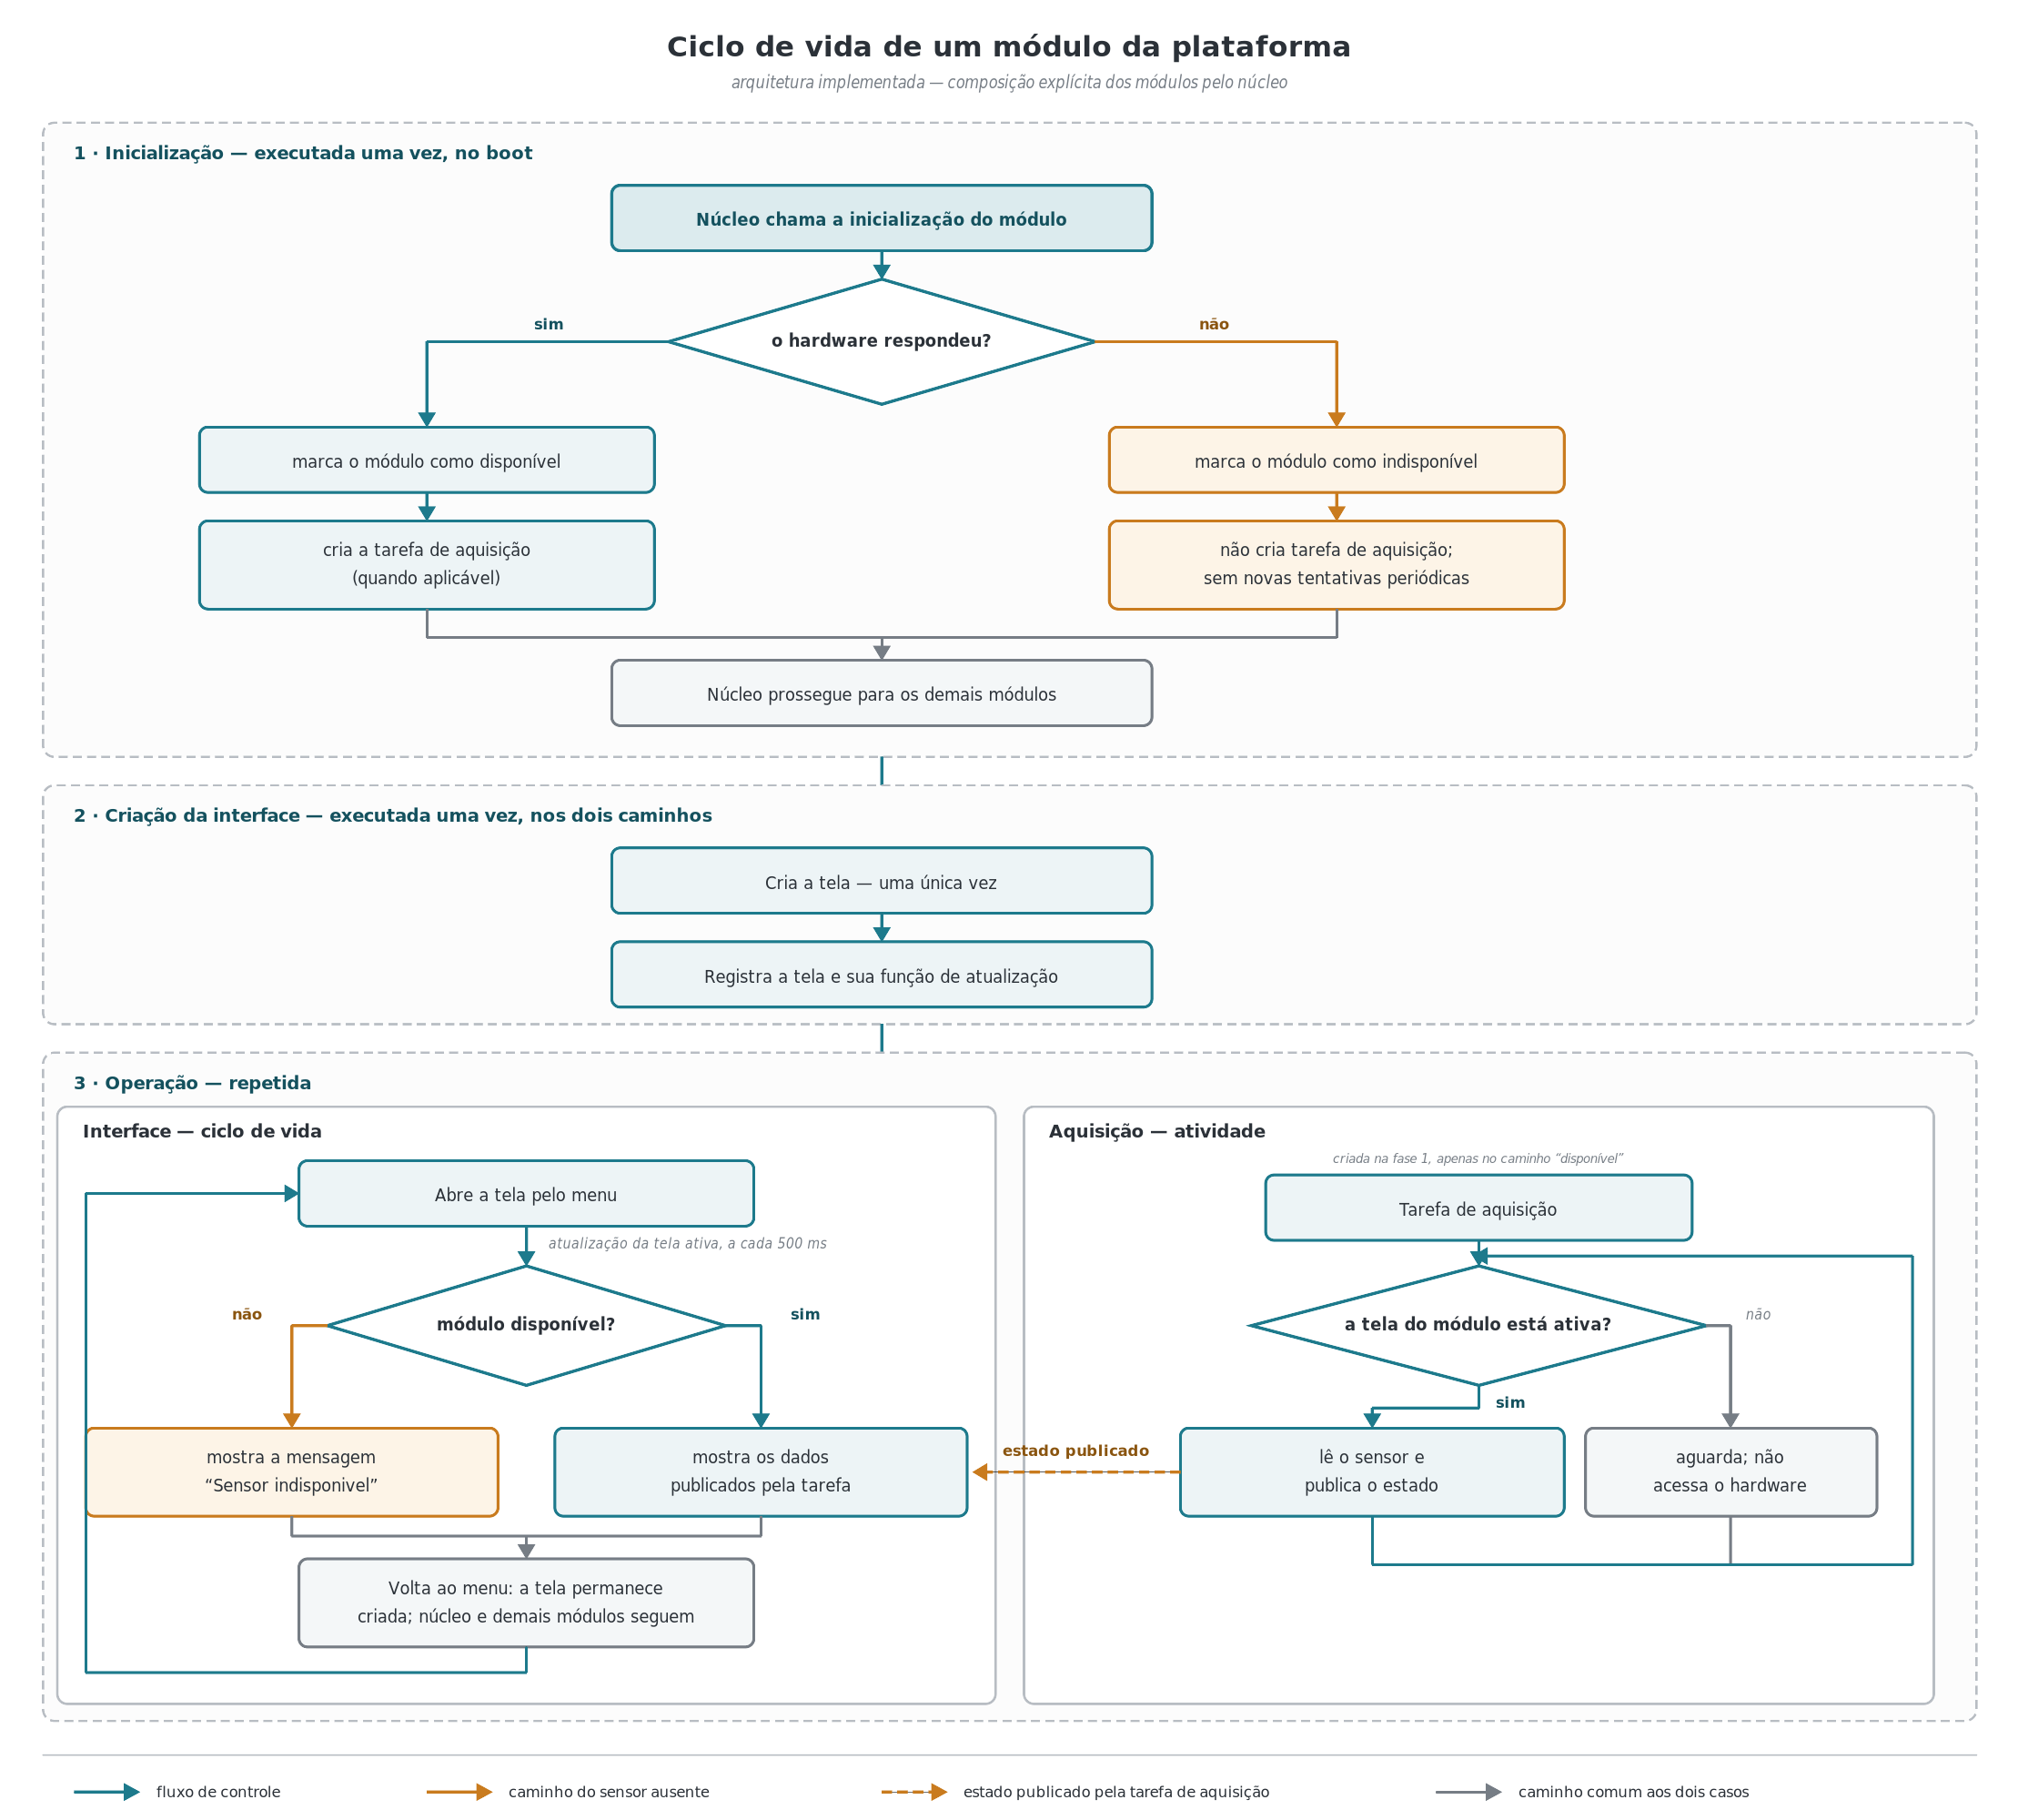
\includegraphics[width=0.94\textwidth]{Diagramas/teoricas/ciclo_vida_modulo.png}
\fonteelemento{Elaborado pelo autor a partir do contrato observado no firmware}
\end{figure}


\subsubsection{Servi\c{c}os do n\'ucleo}


O registro de telas associa um objeto LVGL a uma fun\c{c}\~ao de atualiza\c{c}\~ao. A cada 500 ms, o despachante consulta a tela ativa e chama somente a fun\c{c}\~ao registrada para ela. Menus est\'aticos n\~ao precisam de atualiza\c{c}\~ao peri\'odica, enquanto telas de sensores convertem o estado publicado pelas tarefas em texto, indicadores ou gr\'aficos.


O n\'ucleo tamb\'em concentra a cria\c{c}\~ao do barramento I$^2$C, o scanner de endere\c{c}os, a recupera\c{c}\~ao ap\'os falhas e os estilos compartilhados da interface. O servi\c{c}o \texttt{app\_perf\_read()} fornece uma estimativa explorat\'oria de ociosidade e o heap livre, mas, sem uma s\'erie controlada, esses valores n\~ao foram usados como caracteriza\c{c}\~ao de desempenho.


\subsubsection{Ciclo de vida dos m\'odulos}


Ap\'os a inicializa\c{c}\~ao dos servi\c{c}os b\'asicos, o n\'ucleo percorre os m\'odulos conhecidos. Cada m\'odulo tenta identificar e configurar seu hardware e registra internamente se ficou dispon\'ivel. A cria\c{c}\~ao das telas ocorre mesmo quando um sensor falha, pois a interface precisa apresentar o estado de indisponibilidade sem depender de nova tentativa cont\'inua.


As tarefas s\~ao criadas somente quando necess\'arias ao m\'odulo. Durante a opera\c{c}\~ao, elas alternam entre bloqueio temporizado, aquisi\c{c}\~ao e publica\c{c}\~ao do estado. A tela consome esse estado sem executar diretamente a transa\c{c}\~ao sensorial, evitando que uma atualiza\c{c}\~ao gr\'afica aguarde uma convers\~ao lenta.


Como a composi\c{c}\~ao dos m\'odulos permanece expl\'icita na implementa\c{c}\~ao corrente, a inclus\~ao de um novo sensor exige tanto a prepara\c{c}\~ao do m\'odulo quanto seu registro no n\'ucleo e na interface. A Figura~\ref{fig:integracao-novo-sensor} organiza esse procedimento a partir dos pontos confirmados no firmware.


\begin{figure}[H]
\centering
\caption{Fluxo para integra\c{c}\~ao de um novo sensor ao firmware}
\label{fig:integracao-novo-sensor}
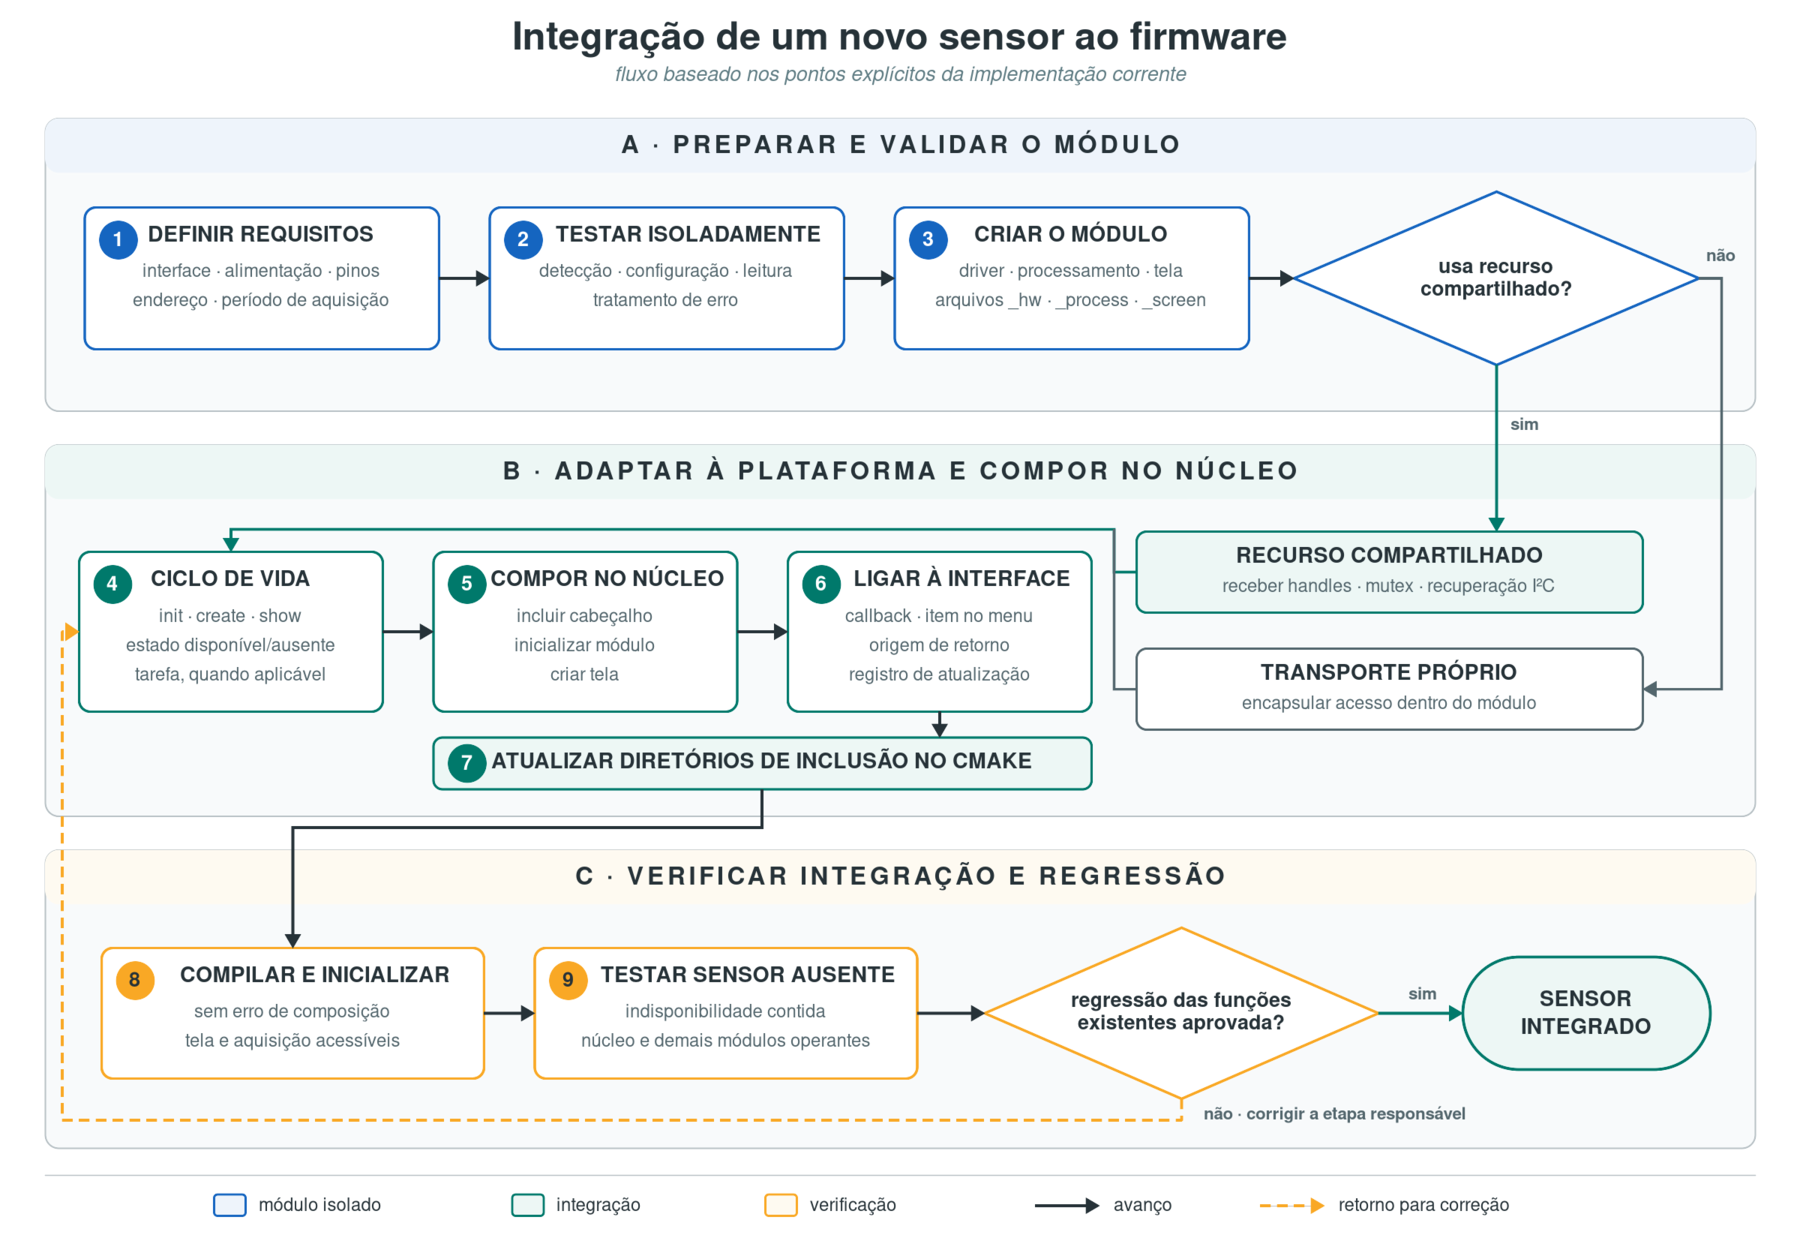
\includegraphics[width=0.95\textwidth]{Diagramas/sistema/integracao_novo_sensor.png}
\fonteelemento{Elaborado pelo autor a partir de \texttt{main.c}, \texttt{app.h}, \texttt{CMakeLists.txt} e da organiza\c{c}\~ao dos m\'odulos sensoriais}
\end{figure}


\subsubsection{Inicializa\c{c}\~ao n\~ao fatal}


A inicializa\c{c}\~ao de um sensor retorna erro ao n\'ucleo, mas esse retorno n\~ao aciona encerramento deliberado da aplica\c{c}\~ao. O m\'odulo marca sua disponibilidade como falsa, preserva uma mensagem apropriada para a tela e n\~ao inicia aquisi\c{c}\~oes que dependam do dispositivo ausente.


O n\'ucleo prossegue com os m\'odulos seguintes e com a cria\c{c}\~ao da interface. Assim, rel\'ogio, toque e sensores presentes podem permanecer dispon\'iveis quando um sensor externo n\~ao responde. A falha de recursos compartilhados, como o pr\'oprio controlador I$^2$C ou o display, possui alcance maior e precisa ser distinguida da aus\^encia isolada de um m\'odulo.


\subsubsection{Modelo de concorr\^encia}


O FreeRTOS opera em configura\c{c}\~ao de n\'ucleo \'unico. A configura\c{c}\~ao padr\~ao usada por \texttt{esp\_lvgl\_port} cria a tarefa gr\'afica com prioridade 4. As tarefas de MAX30102, DS18B20, LTR390, b\'ussola e ped\^ometro s\~ao criadas explicitamente com prioridade 3; a tarefa auxiliar de captura usa prioridade 2; o la\c{c}o de \texttt{app\_main} permanece na tarefa principal do ESP-IDF; e a tarefa ociosa ocupa a prioridade 0.


A frequ\^encia de \emph{tick} foi configurada em 100 Hz, correspondendo a uma resolu\c{c}\~ao de 10 ms. As tarefas aguardam com primitivas de bloqueio e n\~ao realizam espera ocupada entre aquisi\c{c}\~oes. O watchdog de tarefas supervisiona a capacidade de a tarefa ociosa voltar a executar.


As tarefas sensoriais verificam se sua tela est\'a ativa antes de acessar o hardware. Quando a fun\c{c}\~ao n\~ao est\'a em uso, elas bloqueiam por um intervalo e voltam a verificar o estado. Esse condicionamento reduz transa\c{c}\~oes e processamento sem suspender ou destruir repetidamente as tarefas.


A Figura~\ref{fig:tarefas-freertos} organiza as tarefas confirmadas, suas prioridades e os recursos compartilhados.


\begin{figure}[H]
\centering
\caption{Tarefas FreeRTOS e recursos compartilhados no n\'ucleo \'unico}
\label{fig:tarefas-freertos}
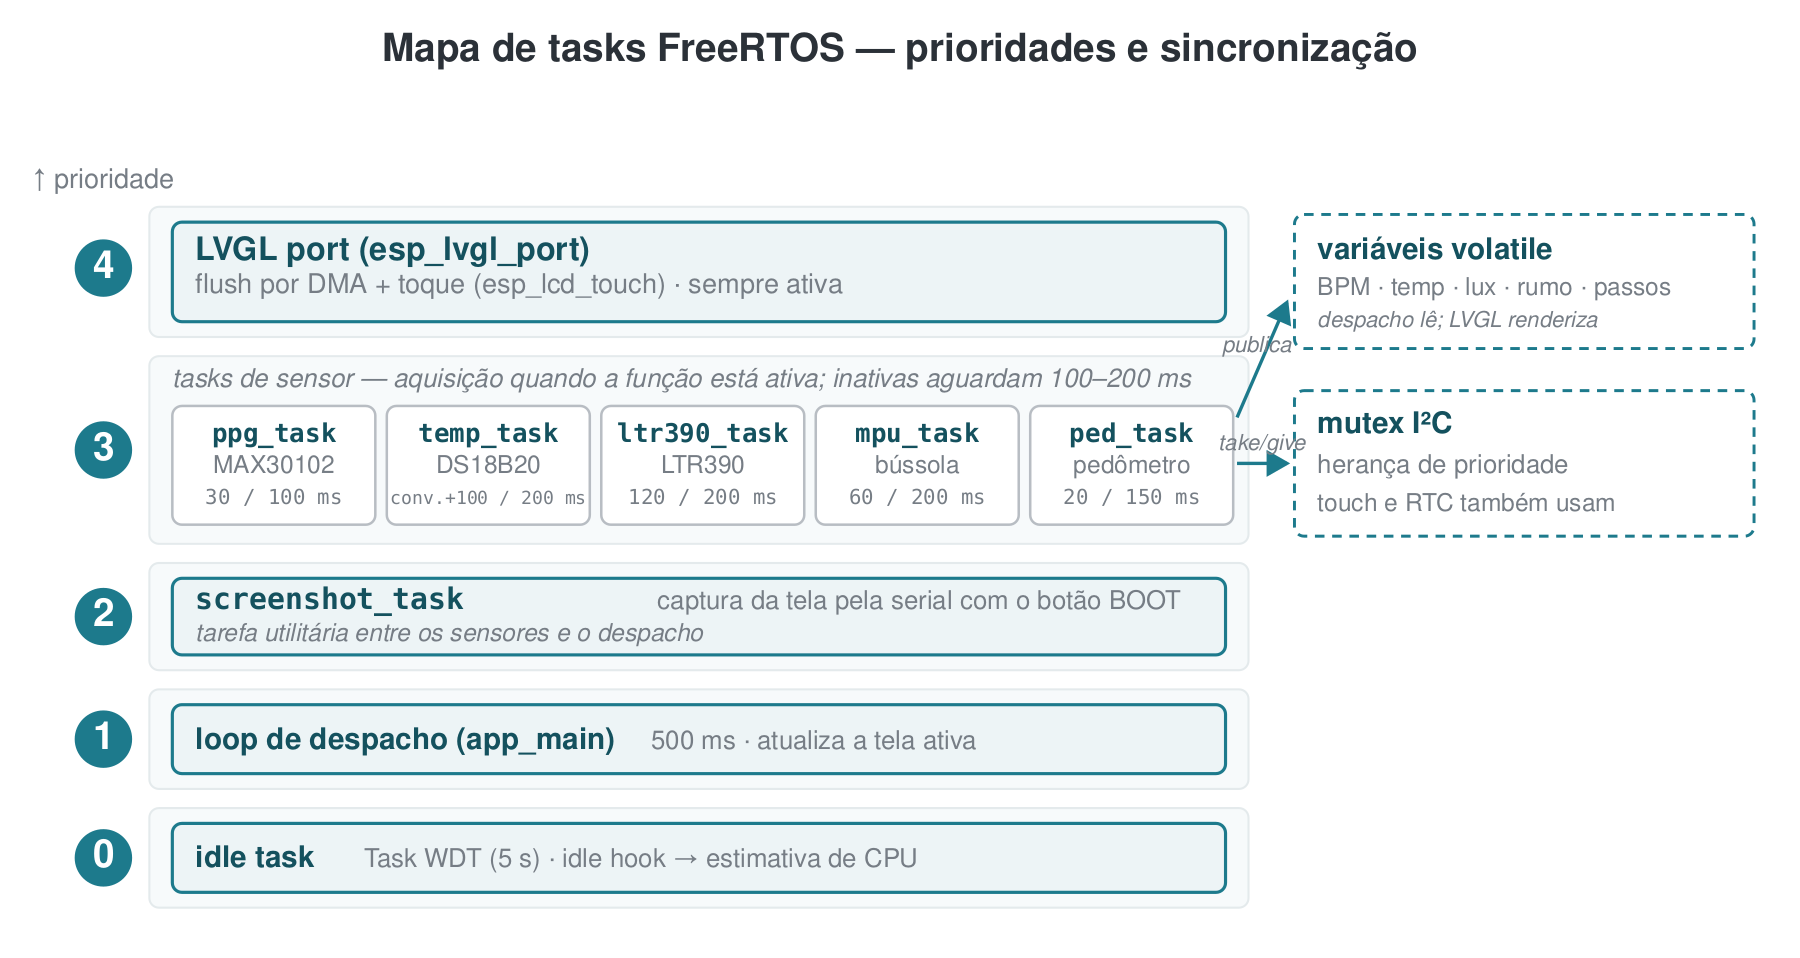
\includegraphics[width=0.98\textwidth]{Diagramas/sistema/freertos_tasks.png}
\fonteelemento{Elaborado pelo autor a partir do firmware e da configura\c{c}\~ao do ESP-IDF}
\end{figure}


\subsubsection{Comunica\c{c}\~ao entre tarefas e interface}


As tarefas publicam as \'ultimas medidas v\'alidas e indicadores de estado em vari\'aveis pertencentes ao m\'odulo. A fun\c{c}\~ao de atualiza\c{c}\~ao da tela l\^e uma fotografia desses valores sob a prote\c{c}\~ao adequada ao tipo de dado. Vari\'aveis escalares alinhadas de at\'e 32 bits podem ser lidas atomicamente pelo processador, mas conjuntos de valores correlacionados exigem cuidado para que a tela n\~ao combine amostras de instantes diferentes.


Apenas o contexto autorizado pela porta da LVGL altera objetos gr\'aficos. Quando uma fun\c{c}\~ao externa ao contexto gr\'afico precisa atualizar a interface, ela obt\'em o bloqueio fornecido pela integra\c{c}\~ao do LVGL. A aquisi\c{c}\~ao permanece independente desse bloqueio para n\~ao reter o recurso gr\'afico durante transa\c{c}\~oes ou processamento.


\subsubsection{Inclus\~ao de novo m\'odulo}


A inclus\~ao de uma nova fun\c{c}\~ao segue uma sequ\^encia definida: implementar ou selecionar o driver; criar o estado e a tarefa, quando necess\'arios; implementar as tr\^es opera\c{c}\~oes do ciclo de vida; registrar a tela e sua atualiza\c{c}\~ao; adicionar o acesso \`a navega\c{c}\~ao. Servi\c{c}os novos somente devem ser acrescentados ao n\'ucleo se forem compartilhados por mais de um m\'odulo ou representarem uma responsabilidade global.


Esse procedimento descreve o ponto de extens\~ao implementado, mas n\~ao quantifica seu custo. O n\'umero de arquivos alterados, as mudan\c{c}as no n\'ucleo e o efeito sobre m\'odulos existentes ser\~ao determinados pelo ensaio de extensibilidade.


\subsection{Robustez do barramento I$^2$C}


\subsubsection{Problema do NACK}


Durante a integra\c{c}\~ao, um NACK deixou de ser apenas um erro local de leitura. Como os dispositivos compartilham controlador e linhas, uma transa\c{c}\~ao interrompida podia afetar a opera\c{c}\~ao seguinte, ainda que destinada a outro endere\c{c}o. Os documentos de desenvolvimento registram ocorr\^encias em que o controlador retornou estado inv\'alido depois da falha inicial.


Cada driver passou a tratar o retorno da API em todas as transa\c{c}\~oes. A aus\^encia de ACK n\~ao \'e interpretada como dado nulo nem ignorada. O m\'odulo recebe o erro, evita publicar uma amostra inv\'alida e aciona o procedimento comum de recupera\c{c}\~ao antes de uma tentativa posterior.


\subsubsection{Mutex com heran\c{c}a de prioridade}


Um mutex \'unico protege as transa\c{c}\~oes do barramento. A tarefa o obt\'em antes da sequ\^encia que deve permanecer indivis\'ivel, executa o acesso e o libera em todos os caminhos de sa\'ida. A prote\c{c}\~ao abrange a transa\c{c}\~ao completa, incluindo sele\c{c}\~ao de registrador e leitura subsequente quando essas etapas formam uma opera\c{c}\~ao l\'ogica.


Foi utilizado mutex, e n\~ao sem\'aforo bin\'ario, para dispor da heran\c{c}a de prioridade oferecida pelo FreeRTOS. Se uma tarefa priorit\'aria aguarda o barramento retido por outra de menor prioridade, a tarefa propriet\'aria pode herdar temporariamente a prioridade at\'e concluir a regi\~ao protegida.


\subsubsection{Recupera\c{c}\~ao do barramento}


O servi\c{c}o de recupera\c{c}\~ao encapsula a chamada \texttt{i2c\_master\_bus\_reset()} oferecida pela API mestre do ESP-IDF (ESPRESSIF SYSTEMS, 2025g). Quando uma transa\c{c}\~ao falha, o driver solicita a recupera\c{c}\~ao ainda dentro do fluxo controlado e somente depois libera o mutex. Dessa forma, outra tarefa n\~ao inicia uma transa\c{c}\~ao enquanto o controlador permanece no estado associado \`a falha anterior.


O reset n\~ao garante que um dispositivo ausente volte a responder. Sua finalidade \'e devolver o controlador e as linhas a uma condi\c{c}\~ao na qual os demais dispositivos possam ser acessados. O n\'umero de tentativas permanece limitado para evitar um ciclo indefinido de falha e recupera\c{c}\~ao.


A ordem do caminho normal e da recupera\c{c}\~ao p\'os-NACK \'e apresentada na Figura~\ref{fig:i2c-recuperacao}.


\begin{figure}[H]
\centering
\caption{Transa\c{c}\~ao I$^2$C e recupera\c{c}\~ao ap\'os falha}
\label{fig:i2c-recuperacao}
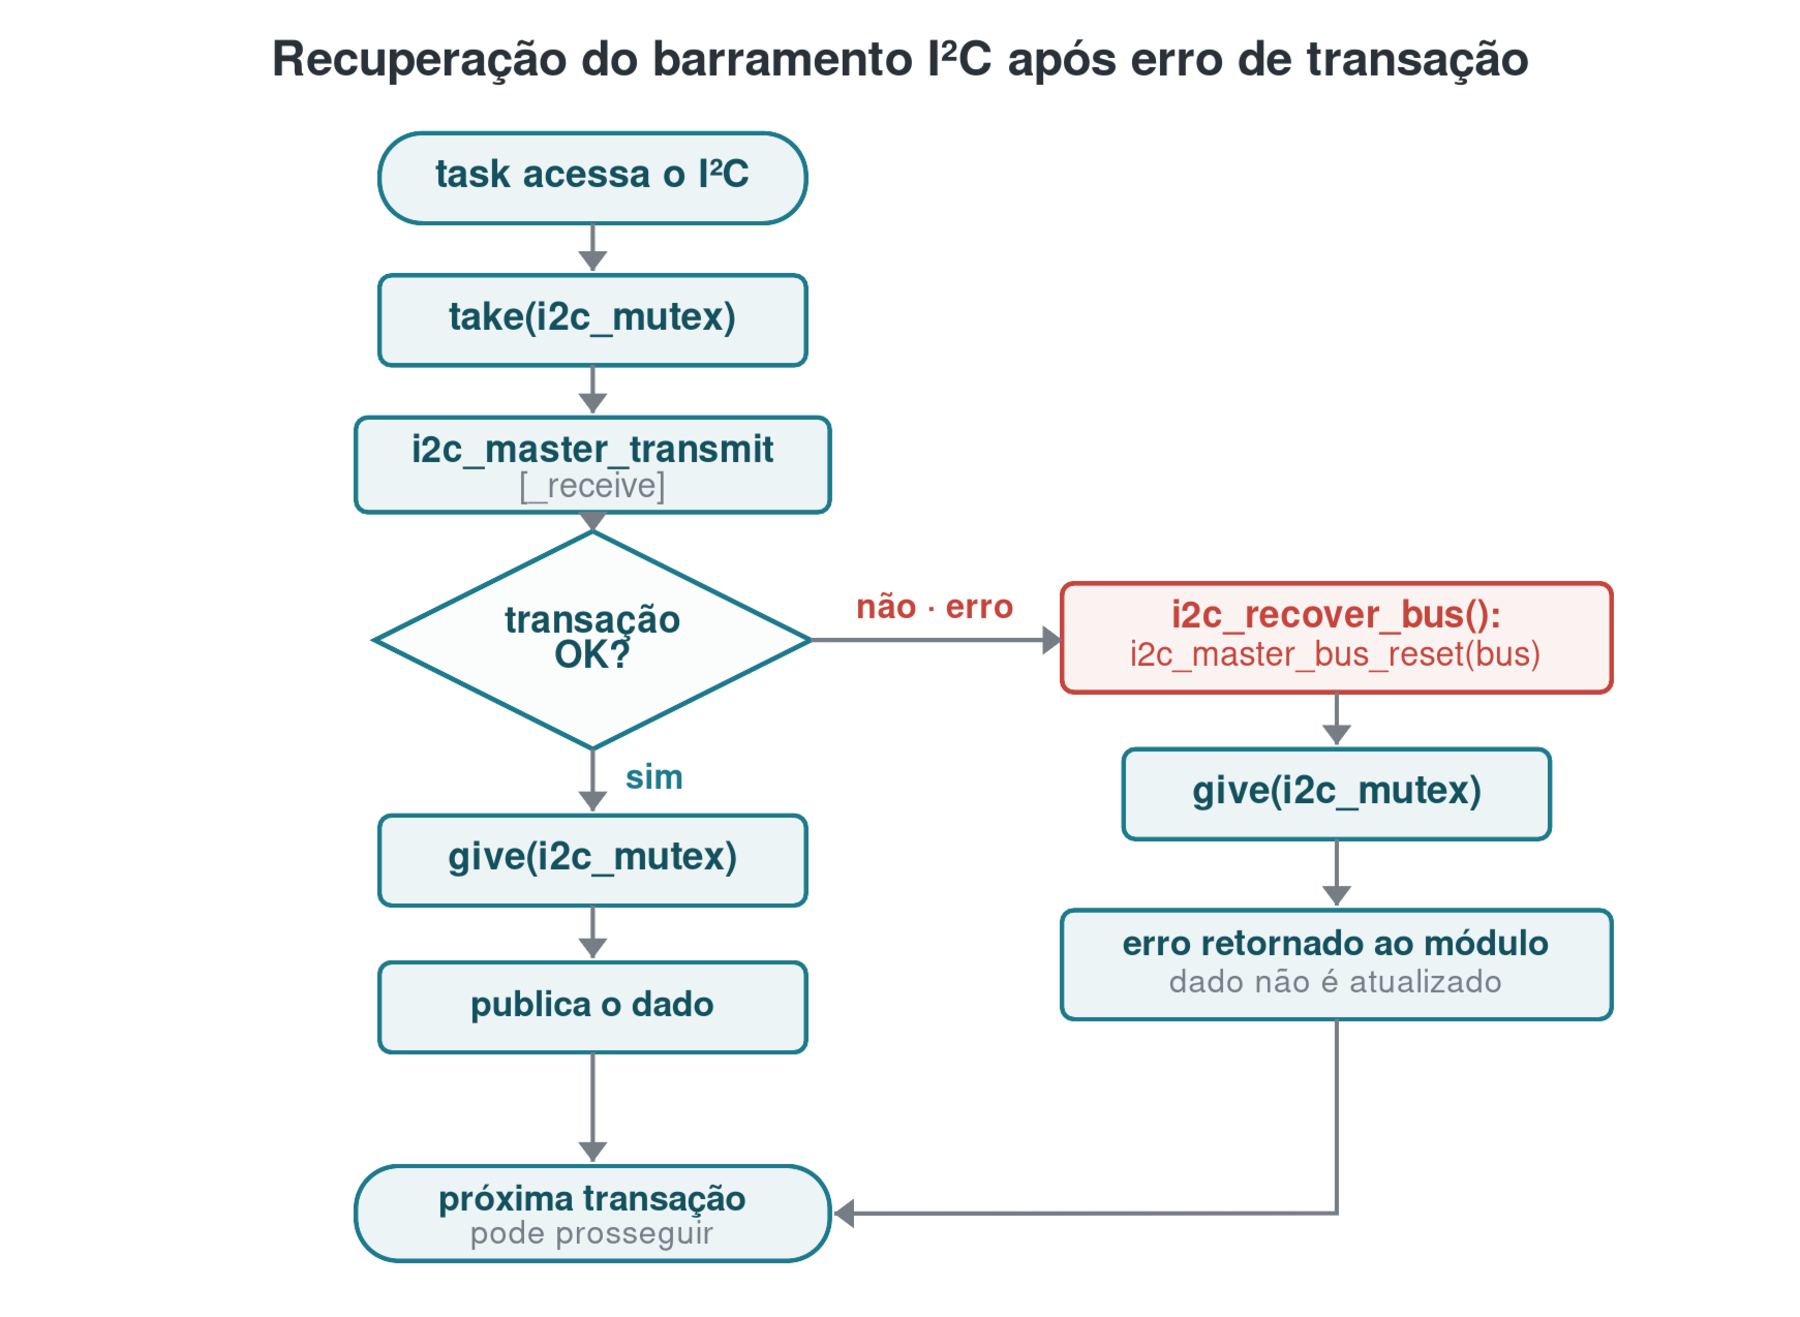
\includegraphics[width=0.94\textwidth]{Diagramas/sistema/i2c_recuperacao_nack.png}
\fonteelemento{Elaborado pelo autor a partir de \texttt{i2c\_recover.c} e dos drivers integrados}
\end{figure}


\subsubsection{Scanner no boot}


Ap\'os criar o barramento, o firmware percorre os endere\c{c}os poss\'iveis e registra os dispositivos que respondem. O scanner foi usado como diagn\'ostico da montagem e permitiu distinguir endere\c{c}o incorreto, sensor ausente e problema geral das linhas.


O resultado da varredura n\~ao substitui a inicializa\c{c}\~ao dos drivers. Responder ao endere\c{c}o demonstra presen\c{c}a no barramento, mas n\~ao confirma identidade, configura\c{c}\~ao nem validade dos dados.


\subsubsection{Redu\c{c}\~ao das transa\c{c}\~oes do touch}


O controlador CHSC6X fornece um sinal de interrup\c{c}\~ao associado ao toque. A primeira integra\c{c}\~ao consultava o dispositivo por I$^2$C mesmo quando n\~ao havia intera\c{c}\~ao. O driver foi alterado para verificar o GPIO17 e iniciar a leitura somente quando o sinal indica evento ativo.


Essa decis\~ao reduz o uso do barramento por uma fun\c{c}\~ao que, na maior parte do tempo, permanece ociosa. A quantifica\c{c}\~ao da redu\c{c}\~ao pertence aos resultados; no desenvolvimento, o aspecto relevante \'e que a interface passou a utilizar uma indica\c{c}\~ao f\'isica de disponibilidade antes da transa\c{c}\~ao.


\subsubsection{Efeito dos logs no sistema}


Mensagens repetidas do driver I$^2$C durante uma sequ\^encia de erros aumentavam o trabalho de formata\c{c}\~ao e transmiss\~ao serial. Em um sistema de n\'ucleo \'unico, essa atividade concorria com a interface e com tarefas temporizadas. Os n\'iveis de log dos componentes mais verbosos foram reduzidos na opera\c{c}\~ao normal, preservando mensagens resumidas e contadores de falha.


Logs detalhados continuam \'uteis em vers\~oes de diagn\'ostico. Sua ativa\c{c}\~ao deve ser tratada como instrumenta\c{c}\~ao capaz de alterar o comportamento temporal, especialmente durante ensaios de CPU, boot e estabilidade.


\subsection{Interface gr\'afica e rel\'ogio}


\subsubsection{Inicializa\c{c}\~ao do display}


O SPI2 \'e configurado antes da cria\c{c}\~ao da interface gr\'afica. O componente do GC9A01A recebe os GPIOs, a frequ\^encia de 40 MHz, a resolu\c{c}\~ao e os par\^ametros de transforma\c{c}\~ao do painel. Ap\'os a sequ\^encia de inicializa\c{c}\~ao, a porta do LVGL associa o buffer de desenho \`a fun\c{c}\~ao de transfer\^encia do controlador.


O conte\'udo foi limitado a uma regi\~ao \'util menor que o ret\^angulo de 240 $\times$ 240 pixels, evitando cortar textos e controles pr\'oximos aos cantos invis\'iveis do painel circular.


\subsubsection{Integra\c{c}\~ao com LVGL}


O \texttt{esp\_lvgl\_port} coordena o temporizador da biblioteca, a entrada por toque e a transfer\^encia das regi\~oes invalidadas. As telas foram constru\'idas com widgets, estilos e fontes, em vez de imagens de quadro completo. Essa estrat\'egia permite alterar valores e indicadores sem armazenar uma imagem integral para cada m\'odulo.


Cada tela \'e criada uma vez e mantida para reutiliza\c{c}\~ao. A navega\c{c}\~ao troca o objeto exibido, enquanto o registro do n\'ucleo seleciona a rotina de atualiza\c{c}\~ao apropriada. Opera\c{c}\~oes que modificam objetos utilizam o bloqueio da porta gr\'afica.


\subsubsection{Corre\c{c}\~ao de cores}


A representa\c{c}\~ao RGB565 exigiu alinhar a ordem dos bytes produzidos pelo LVGL, a ordem dos elementos de cor e a invers\~ao configurada no painel. A configura\c{c}\~ao consolidada combina troca dos bytes de 16 bits, ordem BGR e invers\~ao de cor do controlador.


Esses par\^ametros atuam em n\'iveis diferentes e n\~ao devem ser atribu\'idos somente ao \emph{endianness} do processador. No firmware corrente, \texttt{main.c} define ordem BGR e invers\~ao no controlador, enquanto a op\c{c}\~ao de troca de bytes do RGB565 permanece na configura\c{c}\~ao da LVGL.


\subsubsection{Navega\c{c}\~ao}


A interface utiliza quatro p\'aginas de menu na ordem execut\'avel: sinais vitais, com cora\c{c}\~ao e temperatura; luz e UV; movimento, com b\'ussola e ped\^ometro; e configura\c{c}\~oes de hora e data. A tela principal abre a primeira p\'agina, e as setas laterais percorrem as quatro p\'aginas em sequ\^encia.


A navega\c{c}\~ao \'e independente dos detalhes do sensor. O item conhece a fun\c{c}\~ao p\'ublica usada para exibir a tela, mas n\~ao acessa dados, registradores nem tarefas do m\'odulo.


A Figura~\ref{fig:mapa-navegacao} apresenta os acessos aos m\'odulos, os caminhos de retorno e as telas auxiliares.


\begin{figure}[H]
\centering
\caption{Mapa de navega\c{c}\~ao da interface do prot\'otipo}
\label{fig:mapa-navegacao}
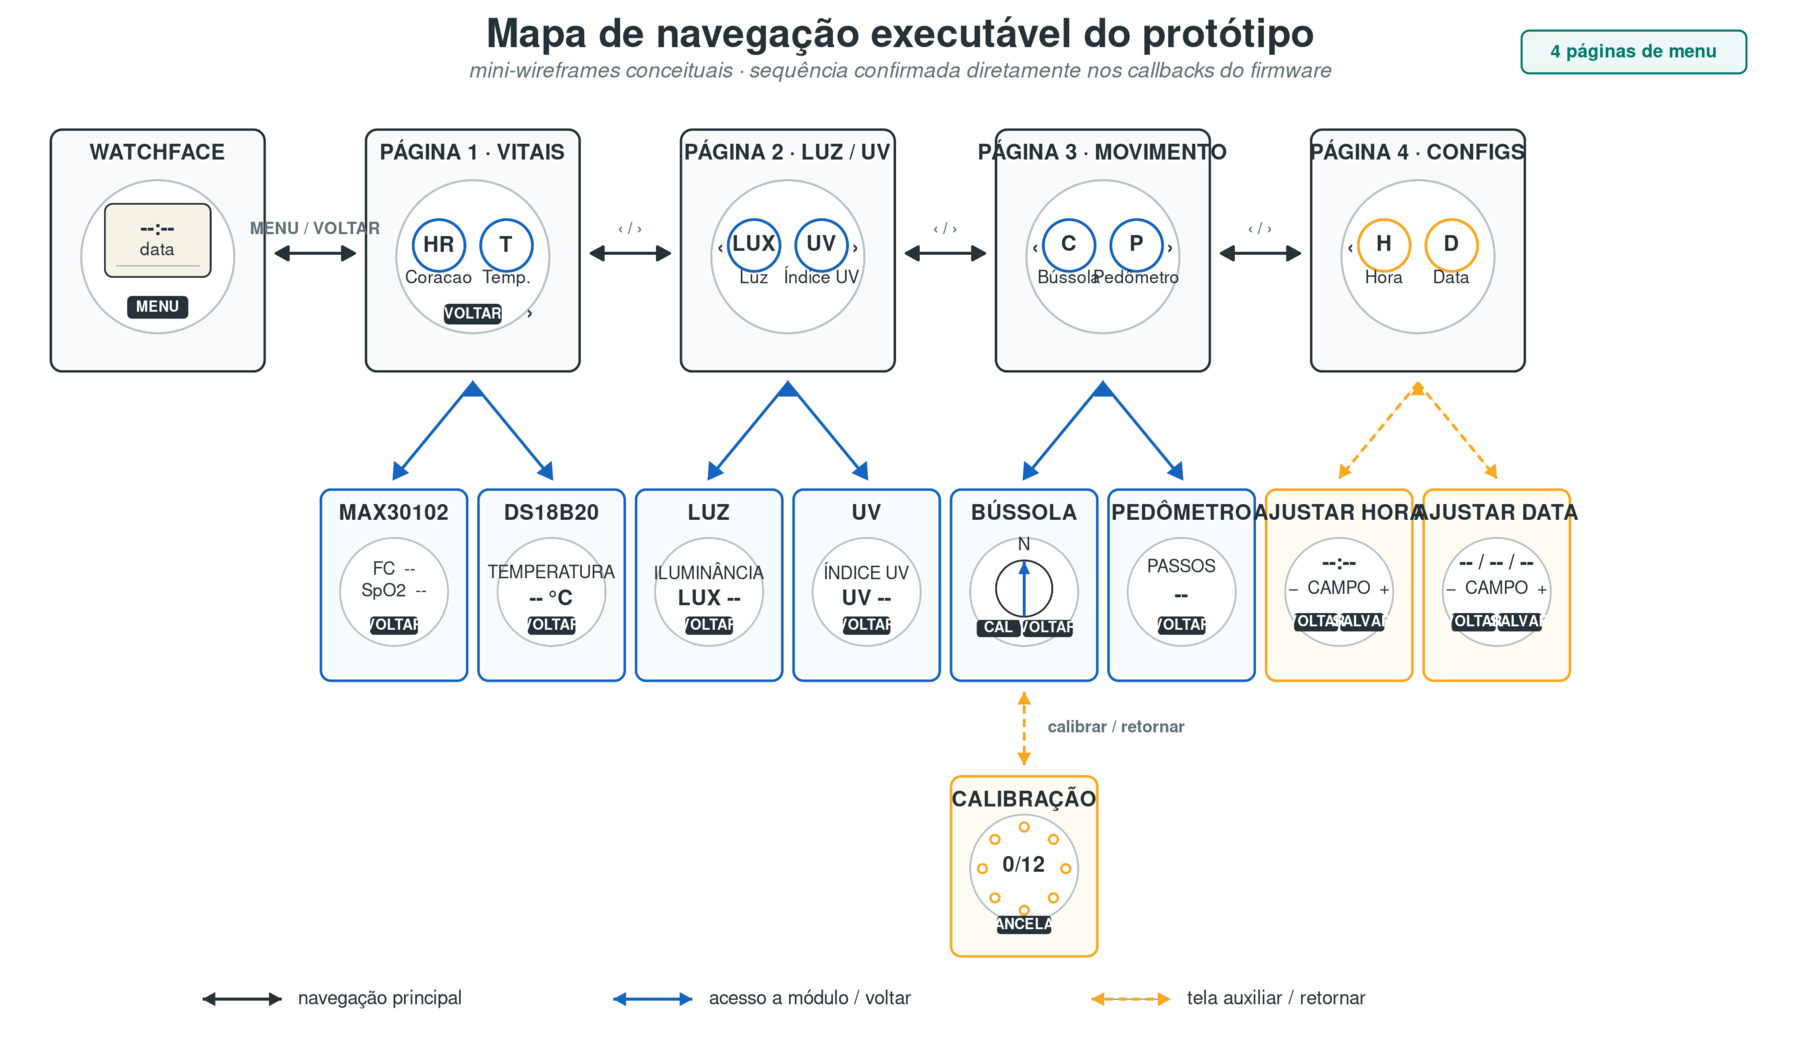
\includegraphics[width=0.98\textwidth]{Diagramas/teoricas/mapa_navegacao.png}
\fonteelemento{Elaborado pelo autor a partir dos \emph{callbacks} e arquivos de tela do firmware}
\end{figure}


\subsubsection{Tela principal}


A tela principal apresenta hora e data obtidas do PCF8563. Um anel de 60 marcadores distribui a indica\c{c}\~ao dos segundos ao redor da circunfer\^encia. Os elementos centrais permanecem dentro do raio \'util e s\~ao atualizados sem reconstruir a tela inteira.


O rel\'ogio tamb\'em oferece o ponto de entrada para a configura\c{c}\~ao de data e hora. A atualiza\c{c}\~ao peri\'odica l\^e os campos necess\'arios do RTC e converte sua representa\c{c}\~ao antes de alterar os r\'otulos.


\subsubsection{Fonte otimizada}


A fonte monoespa\c{c}ada usada na hora foi gerada somente com os algarismos de zero a nove e o caractere de dois-pontos, totalizando 11 glifos. A redu\c{c}\~ao evita incorporar caracteres que n\~ao aparecem naquele r\'otulo.


Como a fonte n\~ao cont\'em espa\c{c}o, o campo ativo na edi\c{c}\~ao n\~ao pode ser ocultado por substitui\c{c}\~ao textual. O firmware varia a opacidade do objeto, mantendo a indica\c{c}\~ao visual sem ampliar o conjunto de glifos.


\subsubsection{Configura\c{c}\~ao por toque}


Dois controles na tela permitem avan\c{c}ar o valor atual e confirmar a etapa. Uma m\'aquina de estados percorre hora, minuto, dia, m\^es e ano. Ao confirmar o \'ultimo campo, o firmware determina o dia da semana e grava o conjunto no PCF8563.


Durante a edi\c{c}\~ao, o campo ativo alterna sua opacidade para indicar qual valor ser\'a alterado. A implementa\c{c}\~ao n\~ao depende de bot\~oes f\'isicos externos ao Round Display.


\subsubsection{RTC PCF8563}


O driver pr\'oprio l\^e sete bytes consecutivos a partir do registrador de segundos. Os valores armazenados em BCD s\~ao convertidos para inteiros e reunidos em uma estrutura de data e hora. Na escrita, o caminho inverso prepara os campos e preserva os bits de controle definidos pelo dispositivo.


O dia da semana \'e calculado a partir da data informada antes da grava\c{c}\~ao. A bateria de reserva do Round Display mant\'em o RTC durante a interrup\c{c}\~ao da alimenta\c{c}\~ao principal. O RTC n\~ao participa da recupera\c{c}\~ao de tempo por rede, pois sincroniza\c{c}\~ao por NTP n\~ao foi implementada.


\subsection{M\'odulo MAX30102}


\subsubsection{Configura\c{c}\~ao}


O driver verifica a identidade do MAX30102 e programa o modo de aquisi\c{c}\~ao dos canais vermelho e infravermelho. A configura\c{c}\~ao corrente utiliza taxa de 100 amostras por segundo, resolu\c{c}\~ao de 18 bits, faixa do conversor de 16.384 nA e corrente aproximada de 7,2 mA em cada emissor. Esses valores correspondem, respectivamente, a 0x67 em \texttt{SPO2\_CONFIG} e 0x24 nos registradores de corrente dos LED.


O componente permanece em \emph{shutdown} quando n\~ao h\'a medi\c{c}\~ao solicitada. A tela oferece um comando de in\'icio, evitando manter os emissores ativos continuamente.


\subsubsection{FIFO e aquisi\c{c}\~ao}


A FIFO desacopla a produ\c{c}\~ao das amostras do instante exato em que a tarefa obt\'em o barramento. A tarefa consulta a quantidade dispon\'ivel, l\^e os bytes em bloco e recomp\~oe cada valor de 18 bits. Os ponteiros da FIFO e condi\c{c}\~oes de transbordamento s\~ao verificados para evitar processar dados incompletos como amostras v\'alidas.


Cada amostra \'e encaminhada ao detector de contato e, quando aceita, \`as etapas de condicionamento. A interface consome apenas os valores publicados pelo processamento, sem drenar a FIFO no contexto gr\'afico.


O fluxo completo, incluindo as portas de aceita\c{c}\~ao que podem rejeitar uma amostra ou um pulso, \'e sintetizado na Figura~\ref{fig:max30102-fluxo}.


\begin{figure}[H]
\centering
\caption{Aquisi\c{c}\~ao e processamento implementados no m\'odulo MAX30102}
\label{fig:max30102-fluxo}
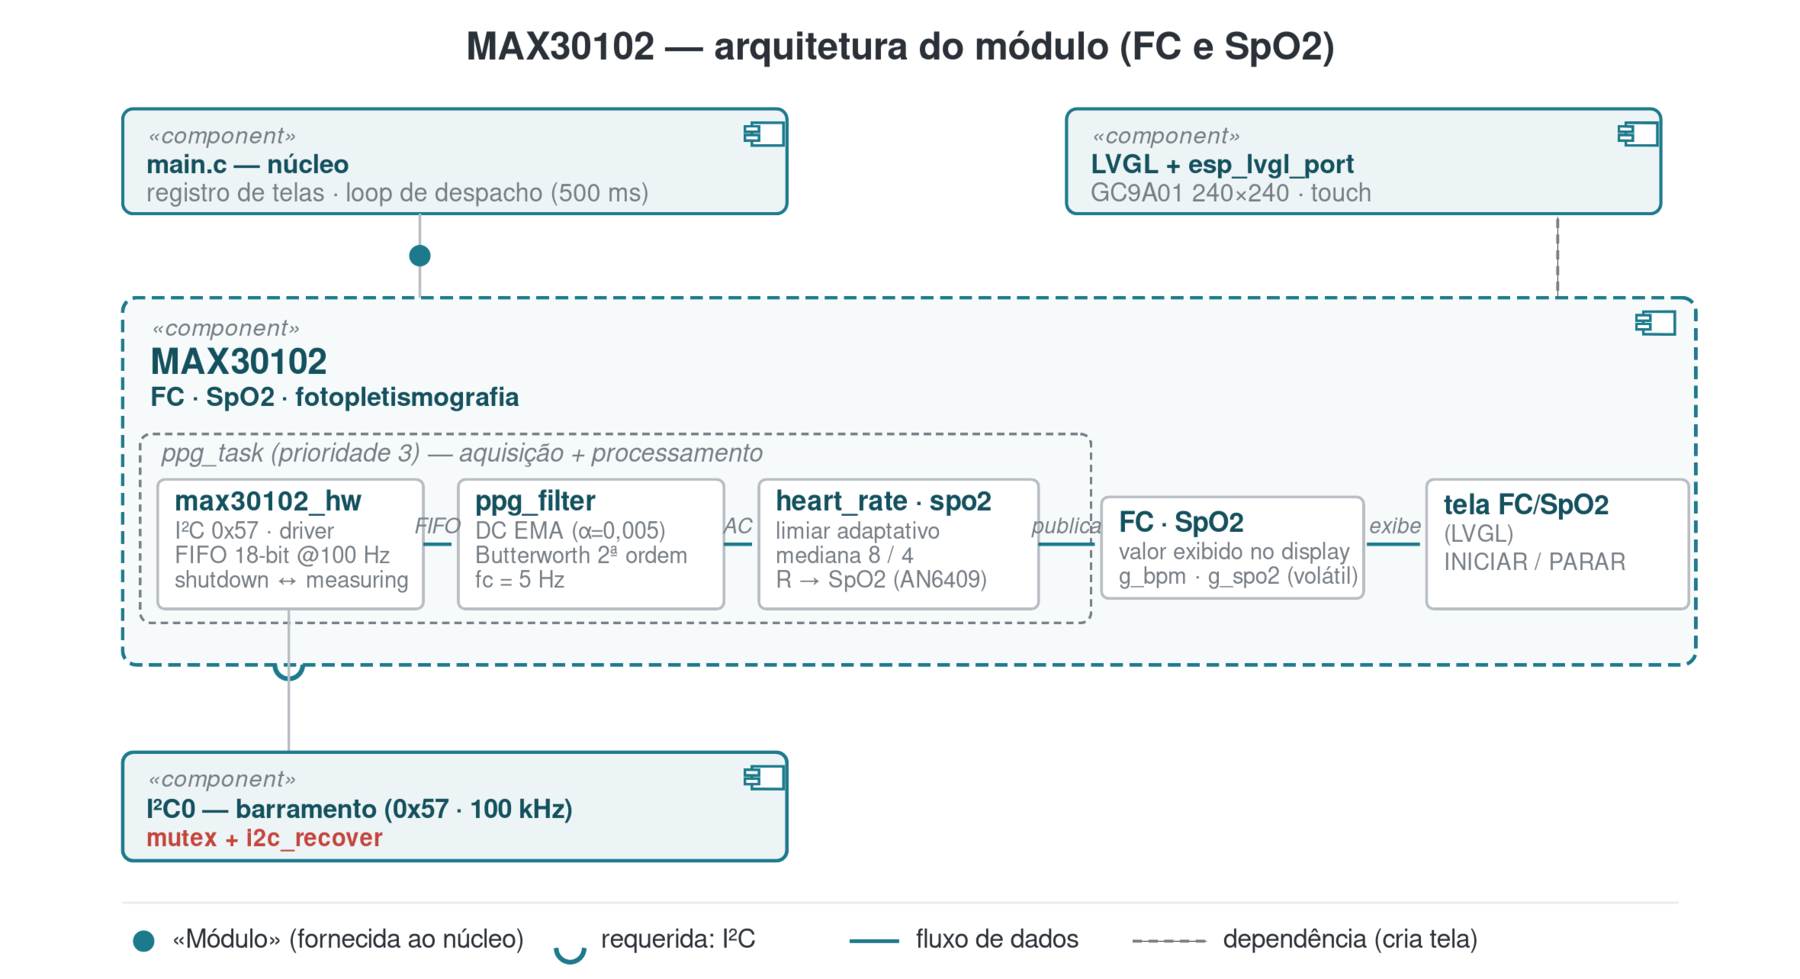
\includegraphics[width=0.96\textwidth]{Diagramas/max30102/max30102_modulo.png}
\fonteelemento{Elaborado pelo autor a partir de \texttt{max30102\_hw.c}, \texttt{ppg\_filter.c}, \texttt{heart\_rate.c} e \texttt{spo2.c}}
\end{figure}


\subsubsection{Detec\c{c}\~ao de dedo}


A presen\c{c}a de contato \'e inferida do n\'ivel do sinal \'optico bruto com limiares distintos para entrada e sa\'ida. A histerese reduz altern\^ancias quando o valor permanece pr\'oximo ao limite. Ao perder contato, o m\'odulo invalida as estimativas e reinicializa estados que n\~ao devem atravessar duas aquisi\c{c}\~oes independentes.


Essa detec\c{c}\~ao indica somente que o n\'ivel \'optico \'e compat\'ivel com contato. Ela n\~ao garante qualidade suficiente para estimar frequ\^encia card\'iaca ou SpO$_2$.


\subsubsection{Filtragem}


Uma m\'edia m\'ovel exponencial acompanha a componente DC. Durante as primeiras 300 amostras, o coeficiente \'e 0,1 para acelerar a estabiliza\c{c}\~ao; depois, passa a $\alpha=0{,}005$. A subtra\c{c}\~ao produz a componente puls\'atil, que passa por um filtro Butterworth de segunda ordem com frequ\^encia de corte de 5 Hz. A frequ\^encia de amostragem usada no c\'alculo dos coeficientes \'e 100 Hz.


Os estados dos filtros s\~ao preservados entre amostras consecutivas e reiniciados quando come\c{c}a uma nova sess\~ao ou quando o contato \'e perdido. O detector ignora as primeiras 500 amostras de cada sess\~ao para que os transientes dos dois est\'agios decaiam antes de publicar batimentos.


\subsubsection{Frequ\^encia card\'iaca}


A detec\c{c}\~ao utiliza uma diferen\c{c}a com intervalo de quatro amostras, o cruzamento de sua derivada associado a um m\'aximo e um limiar adaptativo de amplitude. Candidatos abaixo de 30\% do limiar corrente ou com amplitude absoluta inferior ao limite implementado s\~ao rejeitados. Um per\'iodo refrat\'ario de 400 ms impede que oscila\c{c}\~oes pr\'oximas sejam interpretadas como batimentos distintos.


A frequ\^encia card\'iaca \'e calculada a partir dos intervalos entre batimentos. Uma mediana sobre oito intervalos reduz a influ\^encia de uma detec\c{c}\~ao isolada. Quando n\~ao h\'a quantidade suficiente de eventos v\'alidos, a tela mant\'em a estimativa como indispon\'ivel.


\subsubsection{Estimativa de SpO$_2$}


Para cada batimento aceito, o m\'odulo obt\'em componentes AC e DC dos canais vermelho e infravermelho e calcula a raz\~ao de raz\~oes. A convers\~ao consolidada utiliza a rela\c{c}\~ao emp\'irica


\[
\widehat{\mathrm{SpO_2}}=-45{,}060R^2+30{,}354R+94{,}845.
\]


Crit\'erios de qualidade rejeitam denominadores inadequados, raz\~oes fora da faixa admitida e pulsos com baixa modula\c{c}\~ao. A sa\'ida \'e suavizada pela mediana de quatro estimativas aceitas. O valor permanece denominado estimativa de SpO$_2$, pois a implementa\c{c}\~ao n\~ao passou por valida\c{c}\~ao cl\'inica.


\subsubsection{Invers\~ao dos canais em placas de conex\~ao}


Durante a depura\c{c}\~ao, a ordem observada dos canais em determinadas placas de conex\~ao n\~ao correspondeu \`a atribui\c{c}\~ao inicialmente presumida. Os tr\^es primeiros bytes de cada amostra foram tratados como infravermelho e os tr\^es seguintes como vermelho na montagem utilizada.


Essa corre\c{c}\~ao pertence \`a associa\c{c}\~ao entre o componente e a placa espec\'ifica, n\~ao a uma invers\~ao universal do MAX30102. O driver deve registrar ou encapsular a ordem adotada para impedir que o processamento receba canais trocados.


\subsubsection{Integra\c{c}\~ao com tarefa e tela}


A tarefa do m\'odulo permanece bloqueada quando a tela n\~ao est\'a ativa ou quando a medi\c{c}\~ao n\~ao foi iniciada. Durante uma sess\~ao, ela obt\'em o mutex, drena a FIFO, libera o barramento e executa o processamento. A tela apresenta estado de contato, frequ\^encia card\'iaca e estimativa de SpO$_2$.


Falhas de comunica\c{c}\~ao invalidam a aquisi\c{c}\~ao corrente e acionam a recupera\c{c}\~ao comum do I$^2$C. A interface continua naveg\'avel e diferencia sensor indispon\'ivel, aus\^encia de contato e estimativa ainda n\~ao estabilizada.


\subsection{M\'odulo DS18B20}


\subsubsection{Componente oficial e RMT}


O m\'odulo utiliza os componentes oficiais do barramento 1-Wire e do DS18B20. A cria\c{c}\~ao do barramento informa o GPIO20 e seleciona o RMT como mecanismo de temporiza\c{c}\~ao. O sensor encontrado \'e associado ao componente de n\'ivel superior, que oferece opera\c{c}\~oes de configura\c{c}\~ao e leitura.


Essa reutiliza\c{c}\~ao evita manter no projeto uma segunda implementa\c{c}\~ao dos intervalos do protocolo e da verifica\c{c}\~ao CRC. O m\'odulo permanece respons\'avel pelo ciclo funcional e pela apresenta\c{c}\~ao.


\subsubsection{Ciclo de convers\~ao}


O sensor foi configurado para 11 bits. A tarefa solicita uma convers\~ao, bloqueia durante 375 ms e depois l\^e o \emph{scratchpad}. Esse tempo corresponde \`a resolu\c{c}\~ao selecionada na chamada efetiva de configura\c{c}\~ao.


A espera ocorre por bloqueio da tarefa, e n\~ao por la\c{c}o ativo. Como a temperatura varia lentamente, uma nova convers\~ao s\'o \'e solicitada no per\'iodo definido pelo m\'odulo e quando sua fun\c{c}\~ao est\'a ativa.


\subsubsection{CRC e formata\c{c}\~ao}


O componente verifica o CRC antes de entregar a temperatura. Leituras com erro ou fora da faixa funcional definida para a aplica\c{c}\~ao n\~ao substituem a \'ultima amostra v\'alida. O processamento aplica uma m\'edia m\'ovel exponencial com $\alpha=0{,}5$ e a tela apresenta o resultado com uma casa decimal.


A configura\c{c}\~ao do LVGL adotada n\~ao oferece formata\c{c}\~ao direta de ponto flutuante pela fun\c{c}\~ao usada nos r\'otulos. O m\'odulo converte o valor para d\'ecimos de grau e separa sinal, parte inteira e parte decimal antes de construir o texto.


\subsubsection{Integra\c{c}\~ao com tarefa e tela}


A inicializa\c{c}\~ao do DS18B20 n\~ao recebe o barramento nem o mutex I$^2$C. Depois de encontrar e configurar o sensor, o m\'odulo cria sua tarefa e publica temperatura e estado. A tela l\^e esses dados e apresenta indisponibilidade quando a inicializa\c{c}\~ao ou a leitura falha.


\subsection{M\'odulo LTR390}


\subsubsection{Configura\c{c}\~ao}


O driver adiciona o LTR390 ao barramento no endere\c{c}o 0x53 e a 100 kHz, verifica sua identifica\c{c}\~ao e programa resolu\c{c}\~ao de 18 bits com integra\c{c}\~ao e taxa de 100 ms. A configura\c{c}\~ao associa ganho 3$\times$ ao canal de luz ambiente e ganho 18$\times$ ao canal ultravioleta.


\subsubsection{ALS e UVS}


Os canais ALS e UVS utilizam o mesmo conversor e n\~ao operam simultaneamente. O estado do m\'odulo registra o modo configurado, a disponibilidade de nova amostra e as m\'edias mantidas separadamente para ilumin\^ancia e UVI.


Uma solicita\c{c}\~ao da tela de luz seleciona ALS, enquanto a tela de ultravioleta seleciona UVS. Essa decis\~ao permanece interna ao m\'odulo e n\~ao modifica o n\'ucleo nem o driver de outro sensor.


\subsubsection{Altern\^ancia e estabiliza\c{c}\~ao}


Quando o modo solicitado difere do atual, o driver reconfigura o sensor e o m\'odulo descarta as tr\^es primeiras amostras. O descarte impede que valores produzidos durante a transi\c{c}\~ao sejam publicados como pertencentes ao novo canal.


A tarefa s\'o alterna quando a fun\c{c}\~ao ativa exige outro modo. N\~ao h\'a comuta\c{c}\~ao cont\'inua em segundo plano para manter simultaneamente dois valores que n\~ao est\~ao sendo exibidos.


A Figura~\ref{fig:ltr390-estados} explicita que o modo segue a tela ativa e que os valores somente se tornam v\'alidos para a interface ap\'os o descarte das tr\^es amostras.


\begin{figure}[H]
\centering
\caption{M\'aquina de estados implementada para o LTR390}
\label{fig:ltr390-estados}
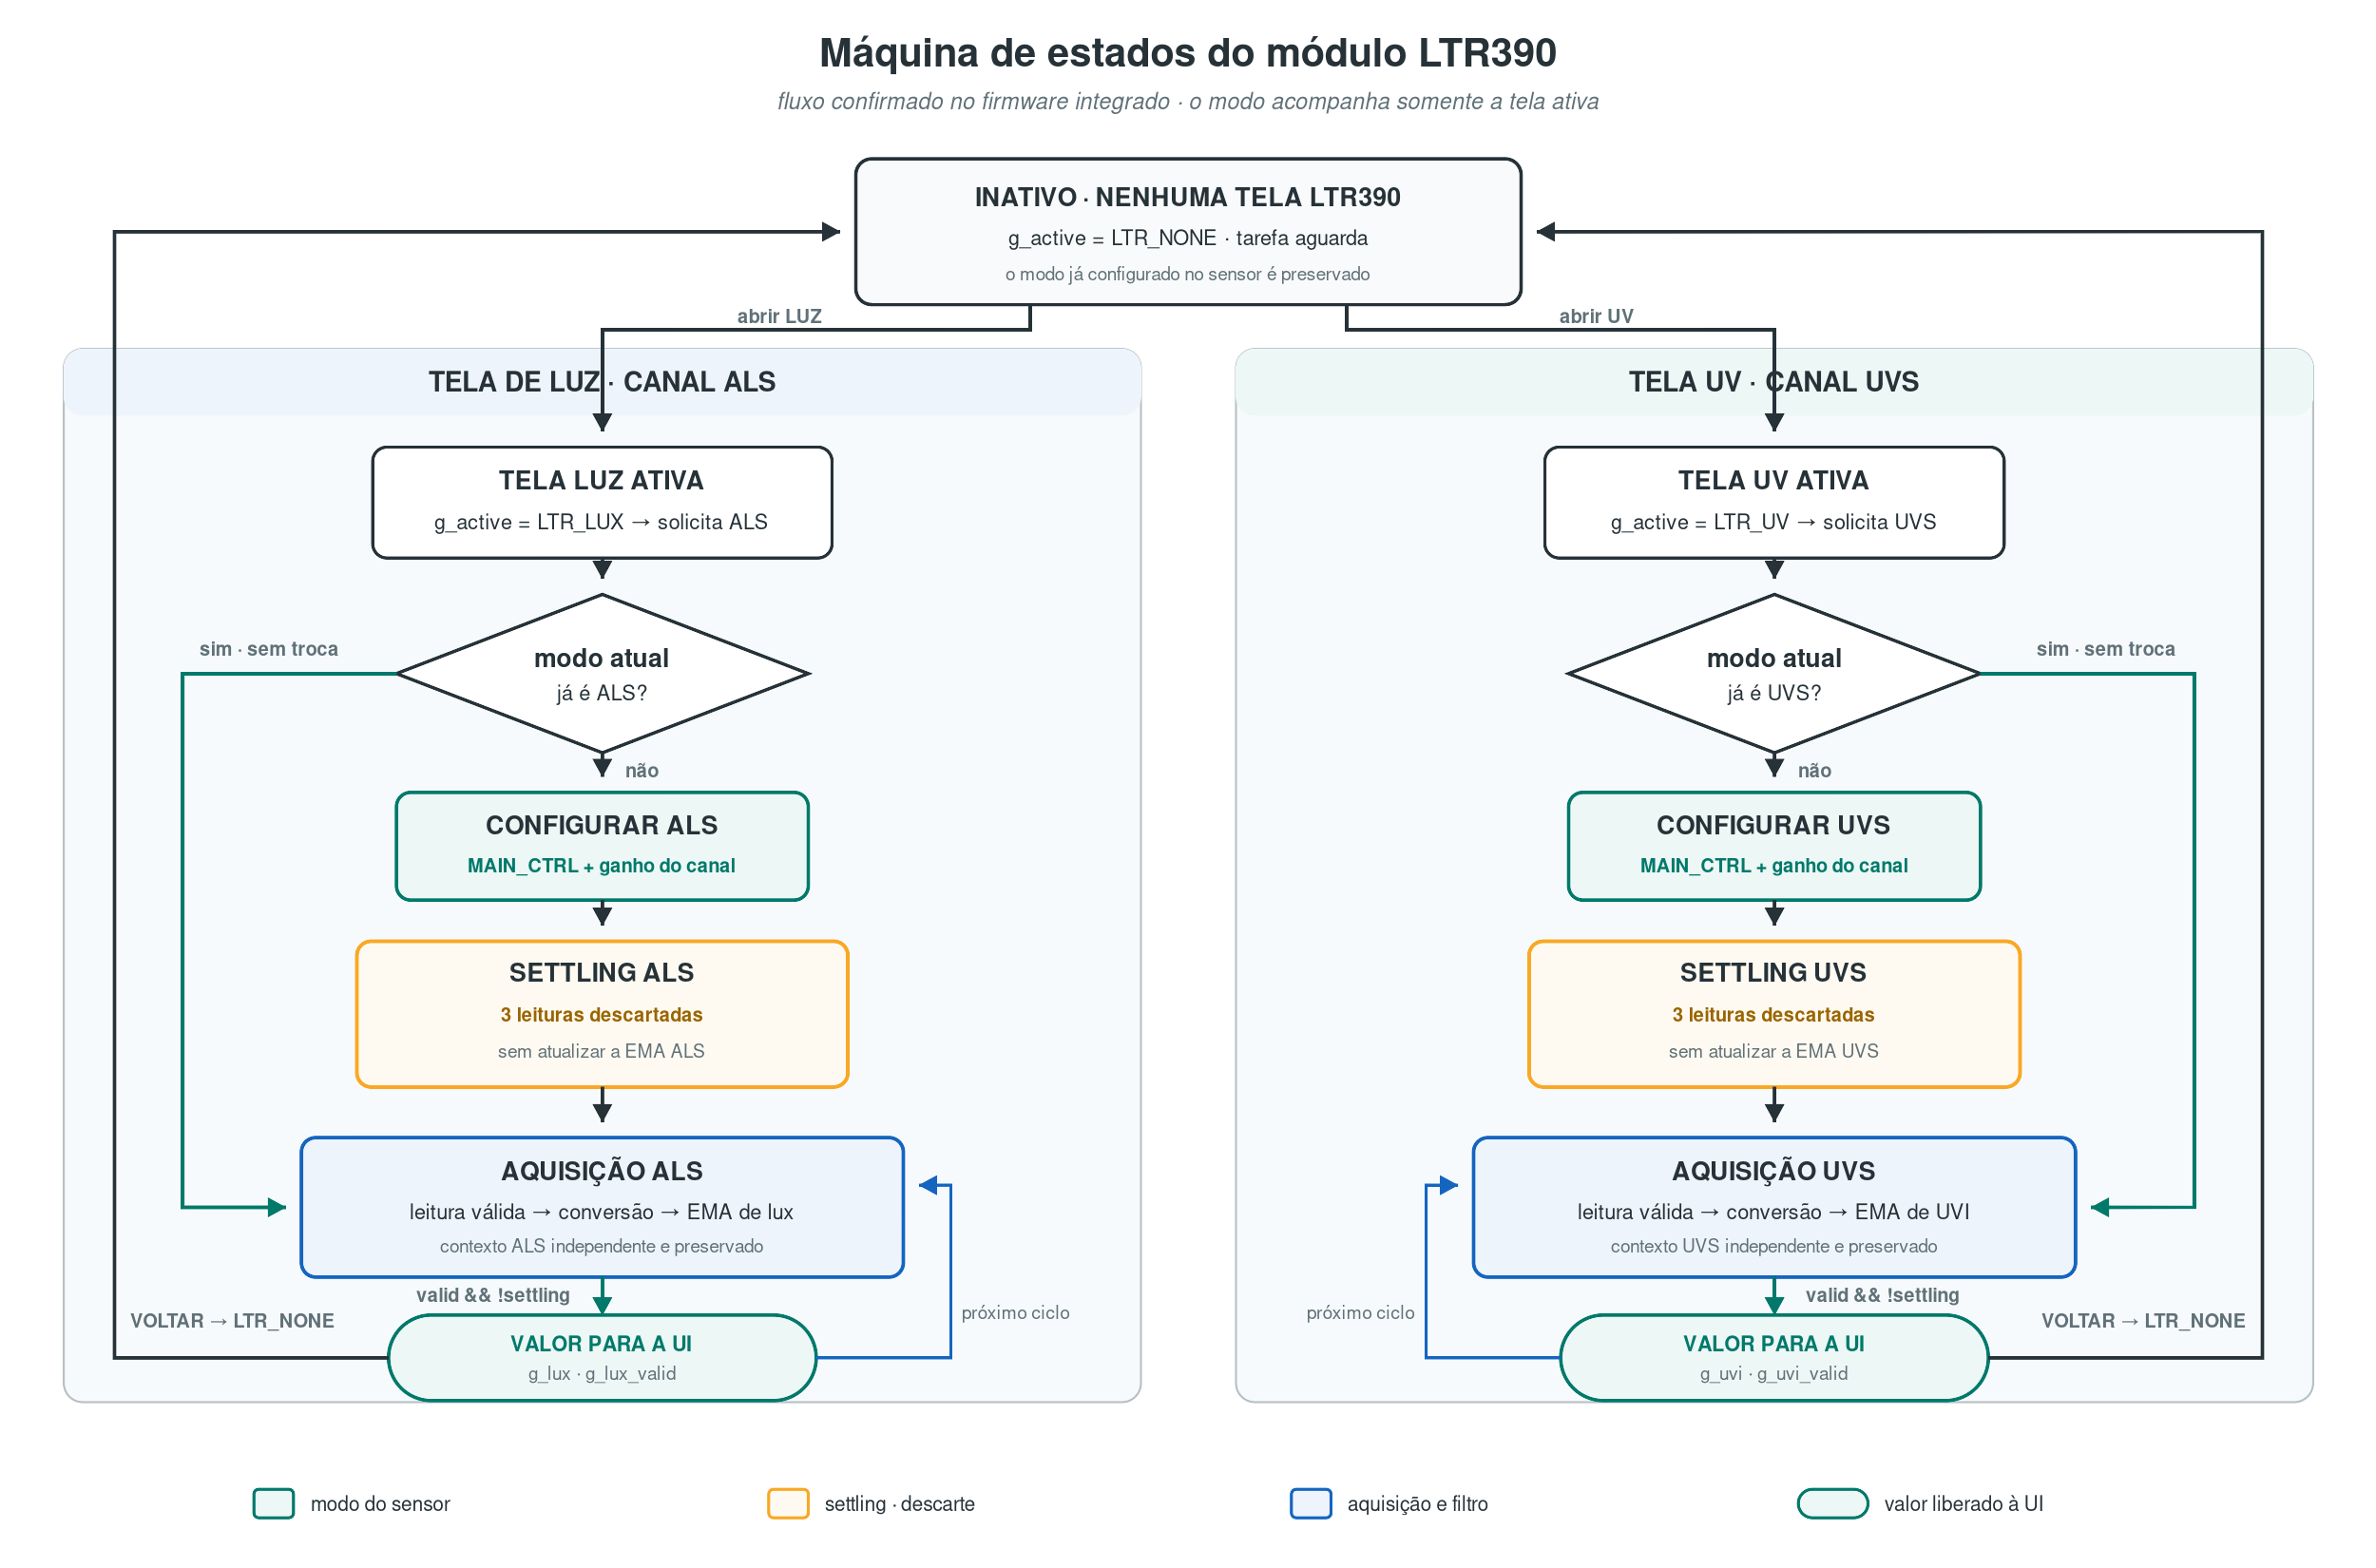
\includegraphics[width=0.98\textwidth]{Diagramas/teoricas/ltr390_maquina_estados.png}
\fonteelemento{Elaborado pelo autor a partir de \texttt{ltr390\_screen.c} e \texttt{ltr390\_process.c}}
\end{figure}


\subsubsection{Convers\~ao para lux e UVI}


Na configura\c{c}\~ao consolidada, a ilumin\^ancia \'e calculada por


\[
E_v=0{,}2\,N_{\mathrm{ALS}},
\]


em que $N_{\mathrm{ALS}}$ \'e a contagem bruta. A estimativa de UVI \'e calculada por


\[
\widehat{\mathrm{UVI}}=\frac{N_{\mathrm{UVS}}}{575}.
\]


Os fatores dependem de ganho e tempo de integra\c{c}\~ao. Por isso, as fun\c{c}\~oes de convers\~ao permanecem associadas \`a configura\c{c}\~ao usada pelo driver e dever\~ao ser atualizadas em conjunto caso esses par\^ametros mudem.


\subsubsection{Remo\c{c}\~ao do SW\_RESET}


A sequ\^encia inicial executava o comando de reinicializa\c{c}\~ao por software. O dispositivo deixava de responder antes de confirmar a escrita, produzindo NACK em uma opera\c{c}\~ao que, no teste isolado, podia parecer apenas uma particularidade local. No barramento compartilhado, esse erro afetava as transa\c{c}\~oes seguintes.


Como todos os registradores necess\'arios j\'a eram programados explicitamente, o comando foi removido da inicializa\c{c}\~ao. A recupera\c{c}\~ao do I$^2$C continua dispon\'ivel para falhas reais, mas n\~ao \'e usada para conservar uma opera\c{c}\~ao desnecess\'aria que produz erro previs\'ivel.


\subsubsection{Integra\c{c}\~ao com tarefa e tela}


A tarefa observa qual das telas do m\'odulo est\'a ativa, configura o modo correspondente, aguarda a estabiliza\c{c}\~ao e publica o valor convertido. Cada canal mant\'em seu estado de filtragem por m\'edia m\'ovel exponencial, com $\alpha=0{,}3$.


Erros de comunica\c{c}\~ao n\~ao s\~ao convertidos em zero. A tela distingue indisponibilidade de uma leitura v\'alida de baixa ilumin\^ancia ou baixa resposta ultravioleta.


\subsection{M\'odulo de b\'ussola}


\subsubsection{Bypass e inicializa\c{c}\~ao}


O driver inicializa o MPU-9250 em 0x68 e habilita o \emph{bypass} para expor o AK8963 em 0x0C ao controlador principal. Em seguida, verifica a identidade do magnet\^ometro e configura seu modo de aquisi\c{c}\~ao. Todo o fluxo utiliza o mesmo mutex e o mesmo servi\c{c}o de recupera\c{c}\~ao dos demais dispositivos.


Na leitura, os registradores de estado s\~ao consultados antes dos dados. O registrador ST2 \'e lido ao final para concluir a sequ\^encia e detectar transbordamento.


\subsubsection{ASA e convers\~ao}


Os coeficientes ASA armazenados de f\'abrica s\~ao lidos no modo apropriado do AK8963. Eles corrigem diferen\c{c}as de sensibilidade entre os eixos e s\~ao aplicados \`a convers\~ao das contagens para microteslas:


\[
m_i=\mathrm{raw}_i\frac{4912}{32760}ASA_i.
\]


O ajuste ASA n\~ao substitui a calibra\c{c}\~ao contra perturba\c{c}\~oes da montagem. Ap\'os essa convers\~ao, o m\'odulo aplica deslocamento e escala obtidos pelo procedimento executado no dispositivo.


\subsubsection{Calibra\c{c}\~ao}


A tela de calibra\c{c}\~ao divide o movimento necess\'ario em 12 setores. Durante a rota\c{c}\~ao do dispositivo, a tarefa acumula m\'inimos e m\'aximos de cada eixo e atualiza a indica\c{c}\~ao de cobertura. Ao concluir os setores, calcula para cada eixo o centro


\[
b_i=\frac{m_{i,\max}+m_{i,\min}}{2}.
\]


e uma escala relativa baseada nas meias-amplitudes observadas. Essa corre\c{c}\~ao representa deslocamento e escala por eixo; n\~ao implementa uma transforma\c{c}\~ao elipsoidal completa com termos cruzados.


O procedimento anterior baseado em exporta\c{c}\~ao CSV foi substitu\'ido pela calibra\c{c}\~ao executada na pr\'opria interface. A vers\~ao final n\~ao exige recompilar o firmware para aplicar novos par\^ametros.


A Figura~\ref{fig:calibracao-ondevice} separa o fluxo acionado pelo usu\'ario do c\'alculo posterior de \emph{heading} e mostra o caminho de cancelamento que preserva a calibra\c{c}\~ao v\'alida.


\begin{figure}[H]
\centering
\caption{Calibra\c{c}\~ao magn\'etica executada no prot\'otipo}
\label{fig:calibracao-ondevice}
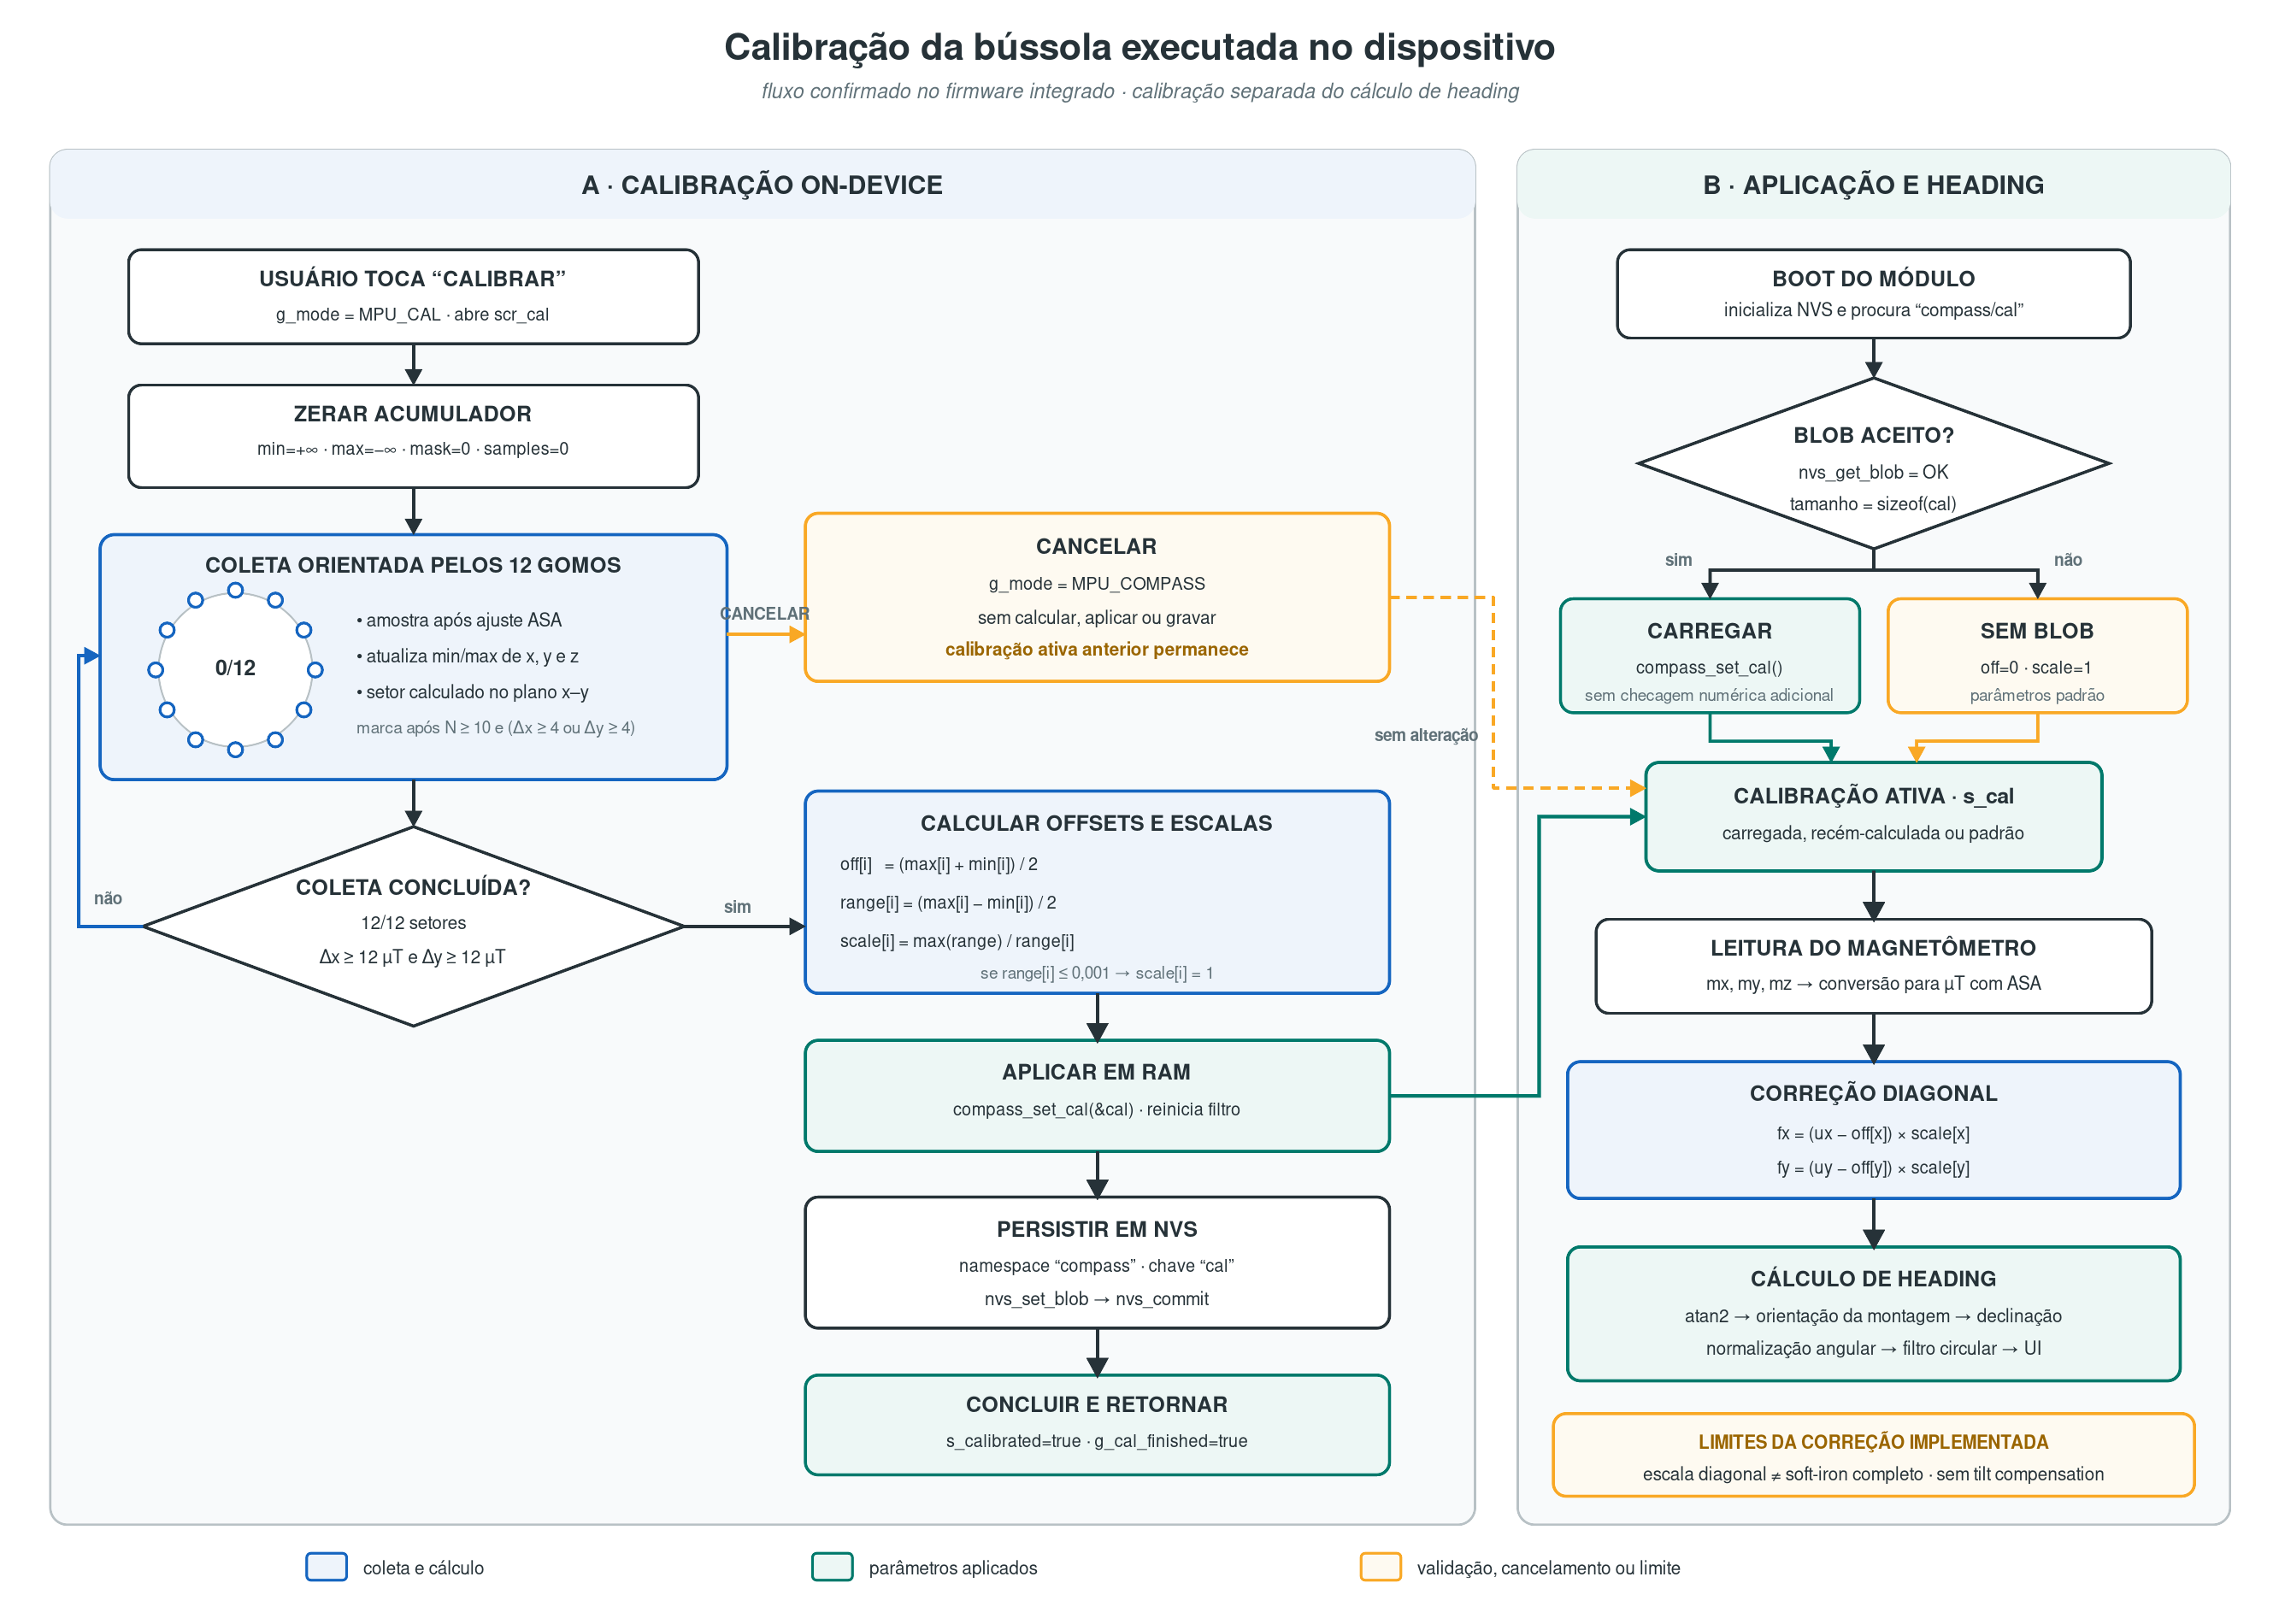
\includegraphics[width=0.98\textwidth]{Diagramas/teoricas/calibracao_bussola_ondevice.png}
\fonteelemento{Elaborado pelo autor a partir do processamento da b\'ussola, da tela de calibra\c{c}\~ao e da persist\^encia em NVS}
\end{figure}


\subsubsection{NVS}


Offsets, escalas e um indicador de validade s\~ao gravados na Non-Volatile Storage (NVS), mecanismo de armazenamento de pares chave-valor em flash fornecido pelo ESP-IDF (ESPRESSIF SYSTEMS, 2025h). Na inicializa\c{c}\~ao, o m\'odulo tenta carregar os valores e utiliza padr\~oes somente quando n\~ao h\'a conjunto v\'alido. Uma calibra\c{c}\~ao conclu\'ida substitui os dados anteriores de forma controlada.


A persist\^encia \'e restrita \`a b\'ussola. O contador do ped\^ometro n\~ao \'e restaurado ap\'os reinicializa\c{c}\~ao.


\subsubsection{Heading e filtro}


Ap\'os aplicar ASA e calibra\c{c}\~ao, o m\'odulo ajusta o mapeamento dos eixos \`a orienta\c{c}\~ao f\'isica da placa e calcula


\[
\psi=\operatorname{atan2}(m_y,-m_x).
\]


O resultado \'e normalizado para o intervalo de 0$^\circ$ a 360$^\circ$. Um filtro com $\alpha=0{,}15$ trata a diferen\c{c}a angular pelo caminho mais curto, evitando uma m\'edia incorreta entre valores pr\'oximos de 359$^\circ$ e 1$^\circ$.


A implementa\c{c}\~ao inverte o sentido de rota\c{c}\~ao devido \`a montagem, acrescenta 180$^\circ$ de orienta\c{c}\~ao f\'isica e aplica declina\c{c}\~ao fixa de $-21^\circ$, conforme os par\^ametros compilados. A tela converte o \^angulo nas oito dire\c{c}\~oes cardeais e intercardeais. N\~ao h\'a compensa\c{c}\~ao de inclina\c{c}\~ao, de modo que a indica\c{c}\~ao pressup\~oe o dispositivo aproximadamente nivelado; a declina\c{c}\~ao fixa tamb\'em deve ser atualizada para outro local ou \'epoca.


\subsubsection{Integra\c{c}\~ao com tarefa e tela}


A tarefa da b\'ussola e a tarefa do ped\^ometro s\~ao distintas, embora ambas acessem o mesmo MPU-9250 por meio do mutex compartilhado. Quando a b\'ussola est\'a ativa, sua tarefa l\^e o magnet\^ometro a cada 60 ms, atualiza o \emph{heading} e responde a comandos de calibra\c{c}\~ao. A tela apresenta \^angulo, dire\c{c}\~ao e estado dos par\^ametros persistidos.


\subsection{M\'odulo de ped\^ometro}


\subsubsection{Tentativa com DMP}


A primeira abordagem procurou utilizar o Digital Motion Processor (DMP) do MPU-9250. Ela exigia carregar firmware no dispositivo por registradores de mem\'oria. Na combina\c{c}\~ao de m\'odulo e implementa\c{c}\~ao testada, esses acessos produziram NACK e impediram concluir a inicializa\c{c}\~ao.


O ocorrido n\~ao demonstra incompatibilidade geral do DMP com o ESP32-C6. Diante do custo de investigar uma depend\^encia adicional e da necessidade de controlar o algoritmo, optou-se por um ped\^ometro implementado no firmware principal.


\subsubsection{Algoritmo pr\'oprio}


O algoritmo utiliza apenas o aceler\^ometro do MPU-9250. O girosc\'opio permanece desligado para essa fun\c{c}\~ao. As amostras dos tr\^es eixos s\~ao convertidas para unidades de $g$, combinadas pela magnitude e processadas por um detector de eventos.


O acesso ao aceler\^ometro fica na camada de hardware do m\'odulo, enquanto filtragem e contagem permanecem na camada de processamento. A tarefa coordena as duas sem transferir essas responsabilidades ao n\'ucleo.


\subsubsection{Configura\c{c}\~ao}


O aceler\^ometro opera na faixa de $\pm2g$, com fator de convers\~ao de 16.384 contagens por $g$, e \'e amostrado a 50 Hz. O per\'iodo de 20 ms \'e compat\'ivel com a resolu\c{c}\~ao de 10 ms do \emph{tick} configurado.


\subsubsection{Magnitude, EMA, limiar e intervalo m\'inimo}


A magnitude \'e calculada por


\[
a_m=\sqrt{a_x^2+a_y^2+a_z^2}.
\]


Uma m\'edia m\'ovel exponencial com $\alpha=0{,}2$ reduz componentes r\'apidas. Um passo \'e reconhecido quando o sinal cruza o limiar de 1,15 $g$, respeitando uma histerese de 0,05 $g$. Depois de uma detec\c{c}\~ao, novos eventos s\~ao ignorados por 300 ms, limitando contagens m\'ultiplas do mesmo movimento.


Os par\^ametros s\~ao fixos e foram escolhidos durante o desenvolvimento. Sua adequa\c{c}\~ao a ritmos e usu\'arios diferentes permanece dependente do ensaio controlado de pedometria.


A arquitetura compartilhada entre b\'ussola e ped\^ometro \'e mostrada na Figura~\ref{fig:mpu9250-modulo}. O detector implementado segue a rela\c{c}\~ao conceitual entre limiar, histerese e intervalo refrat\'ario apresentada na Figura~\ref{fig:pedometro-limiar}, na fundamenta\c{c}\~ao te\'orica.


\begin{figure}[H]
\centering
\caption{Arquitetura do m\'odulo MPU-9250}
\label{fig:mpu9250-modulo}
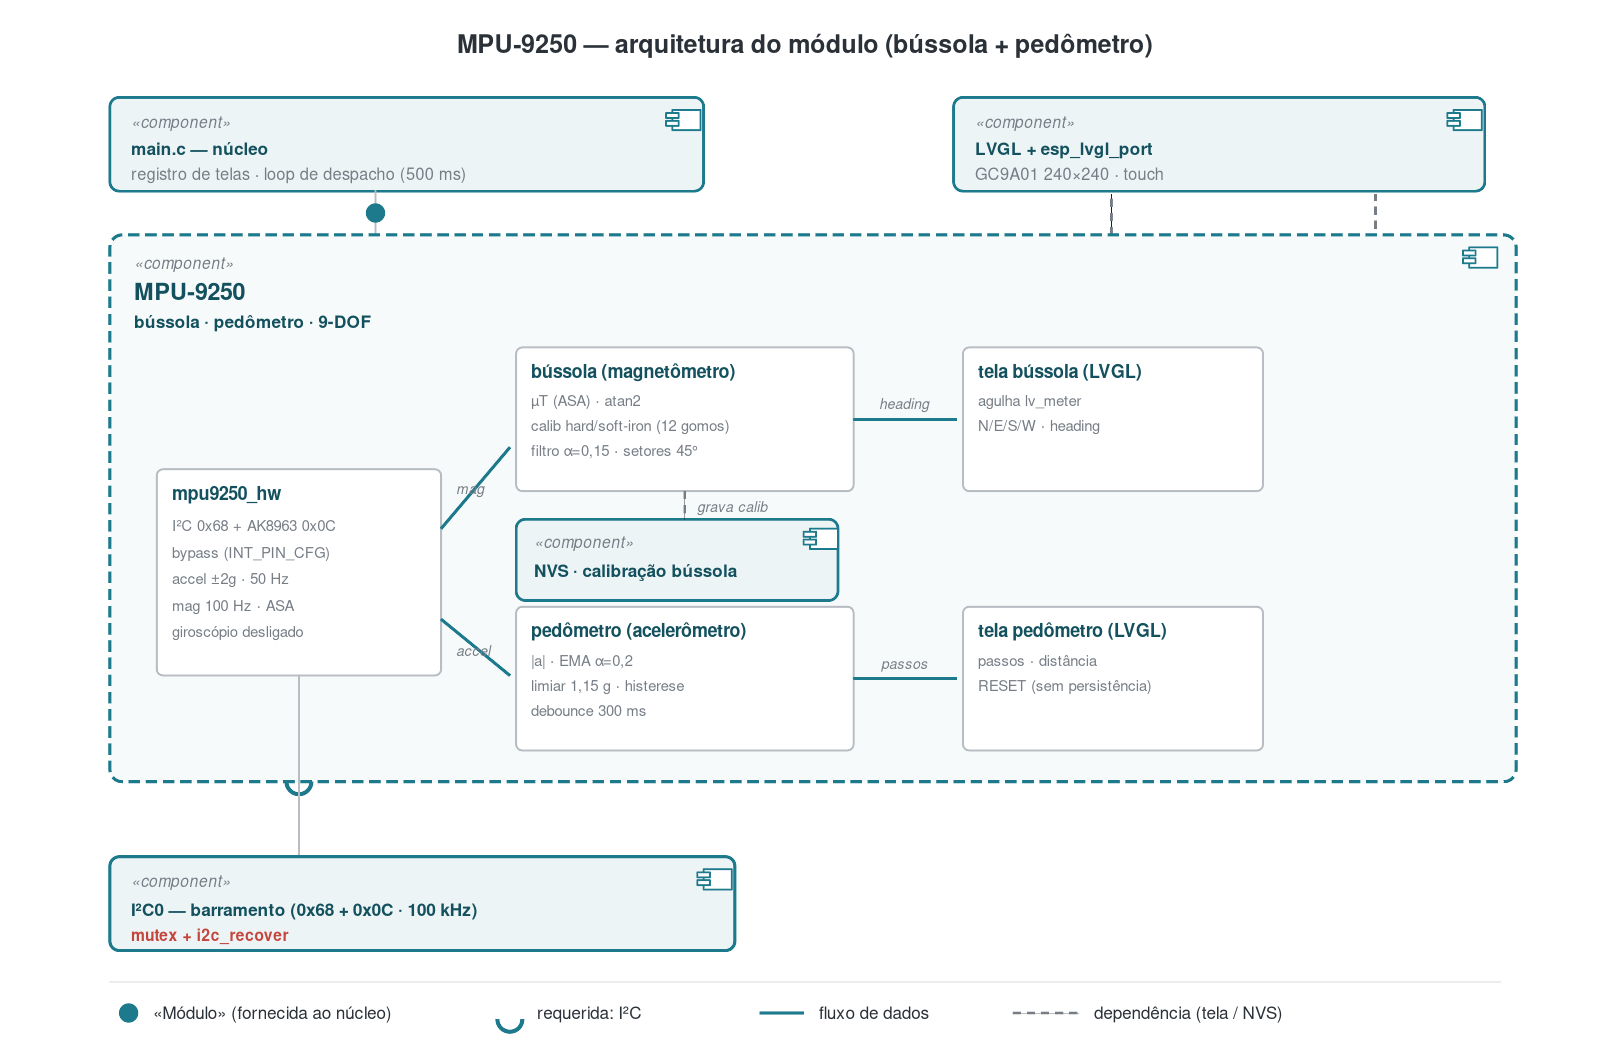
\includegraphics[width=0.96\textwidth]{Diagramas/mpu9250/mpu9250_modulo.png}
\fonteelemento{Elaborado pelo autor a partir de \texttt{pedometer\_process.c} e \texttt{pedometer\_screen.c}}
\end{figure}


\subsubsection{Dist\^ancia estimada}


A dist\^ancia apresentada \'e o produto do n\'umero de passos por um comprimento fixo de 0,70 m:


\[
\widehat d=0{,}70N_{\mathrm{passos}}.
\]


Esse valor n\~ao \'e individualizado por estatura ou padr\~ao de marcha. A interface o identifica como estimativa derivada do contador.


\subsubsection{Integra\c{c}\~ao com tarefa e tela}


A tarefa coleta acelera\c{c}\~ao quando a tela do ped\^ometro est\'a ativa, atualiza o detector e publica passos e dist\^ancia. A tela oferece comando para zerar a sess\~ao. O estado permanece em mem\'oria vol\'atil e retorna a zero ap\'os reinicializa\c{c}\~ao.


\subsection{Uso de mem\'oria e otimiza\c{c}\~oes}


A parti\c{c}\~ao de aplica\c{c}\~ao foi mantida em 1 MiB. A compila\c{c}\~ao limpa da vers\~ao final do bin\'ario produziu um arquivo de 784.240 bytes (765,86 KiB), equivalente a 74,79\% da parti\c{c}\~ao. A contribui\c{c}\~ao incremental de cada m\'odulo ainda n\~ao foi medida por compila\c{c}\~oes controladas.


O pool interno do LVGL foi configurado para 96 KiB. A configura\c{c}\~ao anterior de 32 KiB n\~ao comportava a cria\c{c}\~ao dos objetos da b\'ussola, especialmente o medidor gr\'afico. Esse ajuste aumenta a mem\'oria reservada \`a interface e precisa ser considerado junto ao heap dispon\'ivel.


Uma imagem RGB565 de 240 $\times$ 240 pixels requer ao menos 115.200 bytes sem transpar\^encia; recursos convertidos podem acrescentar cabe\c{c}alho, alinhamento ou outro formato. Para evitar repetir esse custo em cada tela, a interface utiliza widgets, formas e fontes com subconjuntos de glifos.


\subsection{Persist\^encia}


A NVS armazena os par\^ametros de calibra\c{c}\~ao da b\'ussola. O RTC mant\'em data e hora em seu pr\'oprio dom\'inio de alimenta\c{c}\~ao, com bateria de reserva. Esses dois mecanismos possuem ciclos de vida distintos: a NVS conserva par\^ametros do firmware, enquanto o PCF8563 mant\'em a base de calend\'ario.


O ped\^ometro n\~ao possui persist\^encia, e valores instant\^aneos dos sensores n\~ao s\~ao gravados. O projeto tamb\'em n\~ao implementa hist\'orico de medi\c{c}\~oes, armazenamento em cart\~ao microSD ou sincroniza\c{c}\~ao remota. Essas aus\^encias limitam o escopo do estado persistente e evitam atribuir ao prot\'otipo fun\c{c}\~oes de registro que n\~ao foram implementadas.

\end{document}
